%\documentclass[showtrims]{kthesis}
\PassOptionsToPackage{table}{xcolor}
\documentclass[g5paper,twoside,phd,electronic]{kthesis}

%!TEX root = ../main.tex

\usepackage[protrusion=true, expansion=true, final, babel]{microtype}
\usepackage{amsmath}
\usepackage{amssymb}
\usepackage{amsthm}
\usepackage{anyfontsize}
\usepackage{courier} % tt
\usepackage{euler} % math
\usepackage{mathtools}
\usepackage[main=english,swedish]{babel} 
\usepackage[largesc]{newpxtext}
\usepackage{etoolbox}
\usepackage{blindtext}
%\usepackage{makeidx}         % allows index generation
\usepackage{graphicx}        % standard LaTeX graphics tool
\usepackage{multicol}        % used for the two-column index
\usepackage[bottom]{footmisc}% places footnotes at page bottom
\usepackage[normalem]{ulem}	% for strike-through of text with \sout{}  
\usepackage{hyperref}  %for hyperlinks
\usepackage{soul}   % for high-lighting of text
\usepackage{verbatim}
\usepackage{graphicx}
%\usepackage{balance}  % for  \balance command ON LAST PAGE  (only there!)
\usepackage[T1]{fontenc}% Fixes problems with hyphenation
\usepackage{pdfpages}
\usepackage{fancyhdr}
\usepackage{exscale}
\usepackage{booktabs}
\usepackage{multicol}
\usepackage{multirow}
\usepackage{rotating}
\usepackage{xspace}
\usepackage{afterpage,lipsum}
\usepackage{caption}
\usepackage{nicefrac}
\usepackage{paralist}
\usepackage{verbatim}
\usepackage{enumitem}
\usepackage{listings}      % source code
\usepackage{algpseudocode}% http://ctan.org/pkg/algorithmicx
\usepackage{tikz}
\usepackage{array}
\usepackage{relsize}
\usepackage{diagbox}
\usepackage{oubraces}
\usepackage{subcaption}
\usepackage{placeins}
\usepackage{url}
\usepackage{xcolor}
\usepackage[ruled,vlined]{algorithm2e}
\usepackage{amsthm}
\usepackage{ifthen}
\usepackage{pdflscape}
\usepackage{afterpage}
\usepackage{capt-of}% or use the larger `caption` package
\usepackage{todonotes}
\usepackage[numbers]{natbib}
\usepackage{csquotes}
%!TEX root = ../main.tex

\setcounter{tocdepth}{1}
%\setcounter{secnumdepth}{2}

%http://www.tug.org/mactex/fonts/LaTeX_Preamble-Font_Choices.html
% Euler for math | Palatino for rm | Helvetica for ss | Courier for tt
\renewcommand{\rmdefault}{ppl} % rm
\linespread{1.05}        % Palatino needs more leading


\newenvironment{module}[1][htb]
  {\renewcommand{\algorithmcfname}{Specification}% Update algorithm name
   \begin{algorithm}[#1]%
  }{\end{algorithm}}

%hack for urls
\def\UrlBreaks{\do\/\do-\do\/\/}

\definecolor{dkgreen}{rgb}{0,0.6,0}
\definecolor{gray}{rgb}{0.5,0.5,0.5}
\definecolor{mauve}{rgb}{0.58,0,0.82}


\theoremstyle{definition}
\newtheorem{definition}{Definition}[section]

% \theoremstyle{  }

\definecolor{darkred}{rgb}{0.5,0,0}
\definecolor{darkgreen}{rgb}{0,0.5,0}
\definecolor{darkblue}{rgb}{0,0,0.5}

%\usepackage[maxnames=2]{biblatex}
\lstset{frame=l,
  language=Java,
  aboveskip=3mm,
  belowskip=3mm,
  numbers=left,
  firstnumber=1,
  numberfirstline=true
  showstringspaces=false,
  xleftmargin=5pt,
%   framexleftmargin=-1pt,
  columns=flexible,
  basicstyle={\scriptsize\ttfamily},
  %numbers=none,
  numberstyle=\tiny\color{black},
  keywordstyle=\color{blue},
  commentstyle=\color{dkgreen},
  stringstyle=\color{mauve},
  breaklines=true,
  breakatwhitespace=true,
  tabsize=4,
  %for scala
  emph={%  
    object, def, val, zip, window, trigger, evict%
    },emphstyle={\color{blue}\textbf}%
}%



\lstdefinelanguage{scala}{
  morekeywords={abstract,case,catch,class,def,%
    do,else,extends,false,final,finally,%
    for,if,implicit,import,match,mixin,%
    new,null,object,override,package,%
    private,protected,requires,return,sealed,%
    super,this,throw,trait,true,try,%
    type,val,var,while,with,yield},
  otherkeywords={=>,<-,<\%,<:,>:,\#,@},
  sensitive=true,
  morecomment=[l]{//},
  morecomment=[n]{/*}{*/},
  morestring=[b]",
  morestring=[b]',
  morestring=[b]"""
}
%%% optional fonts and color configuration
\SetAlFnt{\sffamily}
\renewcommand\ArgSty{\normalfont\sffamily}
%\renewcommand\KwSty[1]{\textnormal{\textbf{\sffamily#1}}\unskip}
\SetAlCapFnt{\normalfont\sffamily\large}
\renewcommand\AlCapNameFnt{\sffamily\large}
%where did the lines go?
\SetAlgoLined
\SetNlSty{texttt}{}{:}
%-----
\SetKwProg{Fn}{Fun}{}{}
\SetKwProg{Hdl}{Upon}{}{}
\newpage
%tikz libraries
\usetikzlibrary{shapes.geometric}
\usetikzlibrary{arrows}


\newcommand*{\bterm}[1]{\textcolor{blue}{#1}}
\newcommand*{\brterm}[1]{\textcolor{black}{#1}}
\newcommand*{\rterm}[1]{\textcolor{red}{#1}}
\newcommand*{\gterm}[1]{\textcolor{brown}{#1}}

%style macros
\newcommand{\para}[1]{\vspace{2mm}\noindent\textbf{#1}}
\newcommand{\parax}[1]{\noindent\textbf{#1}}
\newcommand{\name}[1]{\textsf{\small #1}}

%math
\newcommand{\CONTRAD}{\Rightarrow\!\Leftarrow}
\newcommand*{\EVT}[1]{\langle {#1} \rangle}

%%%%%%%%%%%%%%%%%%%%%%%%%%%%%%%%%%
%%% SWITCH TODOS ON/OFF HERE %%%%%
%%%%%%%%%%%%%%%%%%%%%%%%%%%%%%%%%%
%\newboolean{commentSwitch}
%\setboolean{commentSwitch}{true}
%%%%%%%%%%%%%%%%%%%%%%%%%%%%%%%%%%
%%%%%%%%%%%%%%%%%%%%%%%%%%%%%%%%%%
%
%\ifthenelse{\boolean{commentSwitch}}{
%  \newcommand{\TODO}[1]{\textcolor{red}{TODO: #1}}
%  \newcommand{\TODOP}[1]{\textcolor{red}{TODO: #1}}
%  \newcommand{\TODOX}[1]{\textcolor{red}{TODO: #1}}
%  \newcommand{\NOTE}[1]{\textcolor{blue}{\textbf{NOTE}: #1}}
%  \newcommand{\DONEX}[1]{\textcolor{blue}{#1}}
%}{
%  \newcommand{\TODO}[1]{}
%  \newcommand{\NOTE}[1]{}
%}
% Margin width for todo notes
\setlength{\marginparwidth}{1.7cm}

%math stuff
\newtheorem{theorem}{Theorem}[section]
\newtheorem{corollary}{Corollary}[theorem]
\newtheorem{problem}[theorem]{Problem}
\newtheorem{lemma}[theorem]{Lemma}


\patchcmd{\abstract}{\titlepage}{\thispagestyle{empty}}{}{}
\patchcmd{\endabstract}{\endtitlepage}{\clearpage}{}{}
\newenvironment{poliabstract}[1]
{\renewcommand{\abstractname}{#1}\begin{abstract}}
  {\end{abstract}}

%!TEX root = ../main.tex

%%
%% This is file `kth-bibl.tex',
%% generated with the docstrip utility.
%%
%% The original source files were:
%%
%% kthesis.dtx  (with options: `biblio')
%%
%% IMPORTANT NOTICE:
%%
%% For the copyright see the source file.
%%
%% Any modified versions of this file must be renamed
%% with new filenames distinct from kth-bibl.tex.
%%
%% For distribution of the original source see the terms
%% for copying and modification in the file kthesis.dtx.
%%
%% This generated file may be distributed as long as the
%% original source files, as listed above, are part of the
%% same distribution. (The sources need not necessarily be
%% in the same archive or directory.)

%============
% TITLE INFO
%============

\title{Scalable Machine Learning through Approximation and Distributed Computing}
\author{Theodore Vasiloudis}
\kthLogo{
\includegraphics{kthlogo}}
\tritaName{TRITA-EECS-AVL}
\tritaYear{2018}
\tritaNumber{54}
\isbn{978-91-7729-901-1}
\monthSubmitted{4}
\defenseDate{2019-09-01}
\defenseTime{11:00}
\defenseHallSwe{Sal A}


\dedication{
  To my parents
}


%\title{Scalable and Reliable Data Stream Processing}
%\author{Paris Carbone}
%\date{August 2018}
%\thesistype{Doctoral Thesis in \\ Information and Communication Technology}
%\imprint{Stockholm, Sweden 2018}
%\examen{teknologie doktorsexamen i datalogi}
%\disputationsdatum{2018-09-28}
%\disputationslokal{Sal A, Electrum, Kungl Tekniska H\"ogskolan, Kistag{\aa}ngen 16, Kista}
%\issn{ISSN xxxx-xxxx}
%\isrn{ISRN KTH/xxx/xx-{}-yy/nn-{}-SE}
%\trita{TRITA-EECS-AVL-2018:54}
%\isbn{ISBN: 978-91-7729-901-1}
%\publisher{Universitetsservice US AB}
%\address{KTH School of Electrical Engineering \\ and Computer Science\\
%  SE-100 44 Stockholm\\
%  SWEDEN}
%\kthlogo{kthlogo}
\endinput
%%
%% End of file `kth-bibl.tex'.


\graphicspath{{./figures/}}



%======================================
% TITLE, CHAPTER, AND SECTION HEADINGS
% by Gabriel
%======================================

\makeatletter
\apptocmd{\@titleFont}{\sffamily}{}{}
\apptocmd{\@frontMatterChapFont}{\sffamily}{}{}
\makeatother

\maxsecnumdepth{subsubsection}

\setlength{\midchapskip}{50pt}
\renewcommand*{\chapterheadstart}{%
  % Remove all space above chapter heading
}
\renewcommand*{\chapnamefont}{%
  \sffamily\large\scshape%
}
\renewcommand*{\chapnumfont}{%
  \normalfont\fontsize{80}{64}\selectfont%
}
\renewcommand*{\printchaptername}{%
  % Do not print 'Chapter' or 'Appendix'
}
\makeatletter
\renewcommand*{\printchapternum}{%
  \flushright%
  \begin{tabular}{@{}c@{}}
    \chapnamefont\MakeLowercase{\@chapapp}\\[.5ex]
    \chapnumfont\thechapter%
  \end{tabular}%
}
\renewcommand*{\printchaptertitle}[1]{%
  \flushleft\chaptitlefont#1%
}
\renewcommand*{\chaptitlefont}{%
  \sffamily\Huge\bfseries%
}
\setsecheadstyle{\sffamily\Large\bfseries}
\setsubsecheadstyle{\sffamily\large\bfseries}
\setsubsubsecheadstyle{\sffamily\bfseries}
\setparaheadstyle{\sffamily\bfseries}

% Customize typesetting of page headers and footers
\newcommand{\hfMarkText}[1]{%
  \footnotesize\textosf{\textsc{\MakeLowercase{#1}}}%
}
\nouppercaseheads
\makeevenhead{headings}%
             {\hfMarkText{\thepage}}%
             {}%
             {\hfMarkText{\leftmark}}
\makeoddhead{headings}%
            {\hfMarkText{\rightmark}}%
            {}%
            {\hfMarkText{\thepage}}
\makeoddfoot{plain}%
            {}%
            {\hfMarkText{\thepage}}%
            {}
\makeatletter
\renewcommand{\@hfMarkText}[1]{\hfMarkText{#1}}
\makeatother

% Remove chapter section numbers from header marks
\addtopsmarks{headings}{}{
  \createmark{chapter}{left}{shownumber}{}{ \ }
}
\addtopsmarks{headings}{}{
  \createmark{section}{right}{shownumber}{}{ \ }
}

% Activate changes
\pagestyle{headings}

% Make new pagestyle where chapter (and no section) appears on both pages
\copypagestyle{headings-chap-only}{headings}
\addtopsmarks{headings-chap-only}{}{
  \createmark{chapter}{both}{shownumber}{}{ \ }
}

% Floor and ceiling
\DeclarePairedDelimiter\ceil{\lceil}{\rceil}
\DeclarePairedDelimiter\floor{\lfloor}{\rfloor}

% Uncertain trees symbols
\newcommand{\calSet}{\ensuremath{\mathbf{C}}\xspace}
\newcommand{\significance}{\ensuremath{\alpha}\xspace}

% Block-GBT symbols
\newcommand{\AND}{\texttt{AND}\xspace}
\newcommand{\bitstring}{\ensuremath{\mathbf{v}}\xspace}

% Paper ordinal numbers
\newcommand{\conceptsicdm}{Paper I\xspace}
\newcommand{\conceptskais}{Paper II\xspace}
\newcommand{\sessionlength}{Paper III\xspace}
\newcommand{\boostvht}{Paper IV\xspace}
\newcommand{\uncertaintrees}{Paper V\xspace}
\newcommand{\blockgbt}{Paper VI\xspace}
%Short versions
\newcommand{\conceptsicdmNum}{I\xspace}
\newcommand{\conceptskaisNum}{II\xspace}
\newcommand{\sessionlengthNum}{III\xspace}
\newcommand{\boostvhtNum}{IV\xspace}
\newcommand{\uncertaintreesNum}{V\xspace}
\newcommand{\blockgbtNum}{VI\xspace}


% GBT formulation
\newcommand{\gbtNumTrees}{\ensuremath{\Kappa}\xspace}
\newcommand{\norm}[1]{\left\lVert#1\right\rVert}


% \raggedbottom
%\input{tex/figure-styles}
%\input{tex/terms}

\begin{document}

\frontmatter
\maketitle
\makecopyright
\makededication
%!TEX root = ../main.tex

\begin{abstract}
Lorem ipsum dolor sit amet, consectetuer adipiscing elit. Mauris
purus. Fusce tempor. Nulla facilisi. Sed at turpis. Phasellus eu
ipsum. Nam porttitor laoreet nulla. Phasellus massa massa, auctor
rutrum, vehicula ut, porttitor a, massa. Pellentesque fringilla. Duis
nibh risus, venenatis ac, tempor sed, vestibulum at, tellus. Class
aptent taciti sociosqu ad litora torquent per conubia nostra, per
inceptos hymenaeos. Aliquam ligula lectus, volutpat in, rutrum sit
amet, ultrices at, elit. Aenean consequat facilisis sapien. Nulla
auctor, wisi vel semper ornare, augue augue facilisis turpis, a
laoreet quam libero quis erat. Vestibulum sagittis. Duis blandit
laoreet tortor. Nulla mattis. Morbi eget turpis. Praesent mi. Nunc
enim leo, blandit ut, sagittis at, pharetra sit amet, dui. Praesent
porta tortor a ligula rutrum dapibus.
\end{abstract}



%!TEX root = ../main.tex

\begin{sammanfattning}

\begin{otherlanguage}{swedish}
	Algoritmer för maskininlärning används i allt högre grad i praktiskt taget alla delar av våra liv. En anledning till deras framgång är förmågan att lära sig komplexa representationer från enorma datamängder. Datorers beräkningshastighet ökar inte lika snabbt som de volymer av data vi vill lära oss från, vilket naturligt leder till algoritmer som måste vara resurseffektiva och parallella.
	I och med att användandet av maskininlärning fortsätter att breda ut sig sig blir förmågan att anpassa sig till en föränderlig värld och att hantera osäkerhet allt viktigare.

	I denna avhandling utvecklar vi skalbara algoritmer för maskininlärning med ett fokus på effektiva distribuerade online-beräkningar. Vi använder oss av \emph{approximationer} för att dramatiskt reducera beräkningskostnaden jämfört med exakta algoritmer, utvecklar algoritmer för \emph{inkrementell inlärning} som hanterar föränderliga miljöer med begränsad beräkningsbudget, samt utvecklar parallella och distribuerade algoritmer som garanterar att våra algoritmer skalar till massiva datamängder.

	Avhandlingen börjar med att beskriva en skalbar algoritm för att beräkna likhet mellan noder i en graf och för att upptäcka begrepp. Vi visar dess användbarhet i flera olika domäner och dess skalbarhet genom att träna på ett av de största tillgängliga text-korpusen på ett fåtal minuter.
	Baserat på en praktiskt tillämpning att prediktera längden på sessioner i media-strömning föreslår vi sedan flertal förbättringar på sätt att träna beslutsträd. Vi beskriver två algoritmer för att skatta osäkerheten för prediktioner gjorda av ``online random forests''. Vår metod uppvisar bättre träffsäkerhet än de bäst presterande metoderna inom forskningsfältet, samtidigt som den tar avsevärt mindre tid att köra.

	Avhandlingen föreslår sedan en parallell och distribuerad algoritm för online träd-boostning som ger samma garantier gällande korrekthet som seriella algoritmer samtidigt som den i genomsnitt är flera storleksordningar snabbare.
	Slutligen föreslår vi en algoritm som tillåter gradient-boostad träning av beslutsträd att distribueras över både datapunkts- och attributs-dimensioner. Vi visar att vi kan reducera mängden kommunikation avsevärt för glesa datamängder i jämförelse med existerande metoder som bara distribuerar beräkningarna längs datapunktsdimensionen och använder täta representationer av datamängder.
\end{otherlanguage}

\end{sammanfattning}



\begin{acknowledgements}


As is always the case in a dissertation, the results this thesis is
a culmination of work and support from multiple people to whom I am
deeply grateful.

First, my academic supervisors, Anders Holst, Henrik Bostr\"{o}m, and Seif Haridi.
They have provided me with guidance and support throughout my thesis and for
that I am grateful.
My industrial supervisor, Daniel Gillblad, has been as good a lab manager and
research colleague as one can hope. His door was always open and he's helped me
grow as a researcher through our joint work and by letting me explore the industry through my
internships. Olof G\"{o}rnerup in many ways taught me how research is done when I
was still starting out, with an eye for detail, creative ideas and an adherence to rigorous
methods.

I want to make special mention of Gianmarco De Fransisci Morales, who
guided me through, from a fledgling PhD student to an independent researcher.
Gianmarco taught me how to insist on the highest standards, provided intuitive
explanations for the most complicated topics, and showed me how one can start
from an idea and transform it to a rigorous paper. This dissertation would
not have been possible without his help.

I've been extremely lucky to work in the industry throughout
my studies and work with people much smarter than me, that I've always learned
from. Boxun Zhang at Spotify, Till Rohrmann at Data Artisans, Hossein Vahabi
at Pandora Radio, and Thomas Drake and Hyunsu Cho at Amazon.
I am deeply grateful for the opportunity to work at all these wonderful
places and for the guidance everyone has provided.

Throughout my studies I've had the chance to talk and learn from some
excellent colleagues here. Paris Carbonne is always around
for a coffee and discussions, be that streaming algorithms or the latest
games. Vasia Kalavri who I'll always look up to for how a PhD should be done.
Anis Nasir for excellent times at conferences and around Stockholm.
Erik Ylip\"{a}\"{a} for our many discussions about everything machine
learning, couldn't have asked for a better office-mate.
Bakr Karali for always finding humor about the life of a southerner
in Sweden. Ian Marsh especially for all the pints, advice, and
emotional support, always there when I needed someone to talk to.
Martin Neumann without whom I would have never had this opportunity,
I'm forever indebted and thankful for the good times over a board game.

Finally, I'm grateful for all my friends. Riccardo and Josh
for PhD life chats and Liene for making sure we talk about other things too.
Kehua, Rado, August, and Jacques, even though you guys left Stockholm I'm grateful for the
good times we had while we were all here. Angelina and Dimitris for unequivocal
support of whatever I chose to do, can't tell you how important that is.
Iraklis and Mitsos for always being there, and keeping me grounded to our
roots.

Last but not least, my parents Vasilis and Erifyli, and my siblings Despina and Kostas.
When everything else goes away, we still have each other.

\end{acknowledgements}

\tableofcontents*
\listoffigures
\listoftables
\listofalgorithms
%\listofacronyms
\mainmatter
\chapter{Introduction}

\newpage
\part{Background}
\label{part:bg}
\chapter{Parallel and Distributed Machine Learning}
\label{ch:bg-parallel-ml}

As the size of the datasets to learn from have grown, so has the need for methods that
can scale and learn from massive data. With the slowdown of CPU frequency
growth, the main avenue for better utilizing modern hardware is to make use
of parallelism, whether that is in a single-worker, or distributed,
making use of a cluster of computers to train models. In this chapter we
will provide an introduction to the systems that make
parallel learning possible and efficient. We start by presenting the
different parallelization paradigms available in Section \ref{sec:bg-ml-paradigms},
continue by presenting the different methods of communicating in
distributed machine learning in Section \ref{sec:bg-ml-communication},
and finish the chapter by highlighting some challenges in
distributed learning in Section \ref{sec:bg-ml-challenges}.
For an in depth look into parallel and distributed Machine Learning (ML)
system design we refer the reader to \cite{distributed-ml-design}.

\section{Parallelization Paradigms}
\label{sec:bg-ml-paradigms}

In an abstract representation of any machine learning problem, we can separate
two functional items: the data, and the model. The data refers to the potentially
massive set, or stream, of data from which we try to learn, be that a labeled dataset for
supervised learning, or an unlabeled dataset from which we try to extract
structure in unsupervised learning. The model refers to the approximate representation
of the real-world process that we use to encode the information about the world,
through the available data.

These two items provide us with a clean separation of how to perform
parallel learning: we can either try to parallelize our learning over the set
of data, known as \emph{data-parallel} learning, or over different parts of
our model, known as \emph{model-parallel} learning. Certain kinds of models
may be more amenable to data or model parallelism. For example, training
linear models using stochastic gradient descent lends itself well to
data-parallel approaches~\cite{dekel-optimal-distributed}, while random
forest (RF) models allow for easy model-parallel learning,
since every tree in an RF can be grown independently.

Finally, it is also possible to employ data and model parallelism simultaneously,
often referred to as block-parallelism, as done by the Latent Dirichlet Allocation
model of \cite{petuum}.

In our work we employ data-parallel learning for Papers \conceptsicdmNum--\sessionlengthNum,
model-parallel learning for Papers \uncertaintreesNum and \boostvhtNum, and
block-parallel learning for \blockgbt. In the sequel we describe and provide
examples of each learning approach.

\subsection*{Data-parallel Learning}
\label{sec:bg-data-parallel}

Data-parallel learning is the most commonly applied form of parallelism
in machine learning models due to the base assumption of many ML models
that the training data are independent and identically distributed (i.i.d.)
\cite{distributed-ml-design}. When performing data-parallel training, we
distribute the data over a set of workers, each of which trains the model
on its own partition of the data. At the end of each iteration there is commonly one communication step
to synchronize the models of each worker to avoid diverging models, although
this requirement can be relaxed, for example for asynchronous gradient descent
algorithms like Hogwild \cite{hogwild} or through the use of stale-synchronous
communication~\cite{stale-sync-ps}.

As \citet{distributed-ml-design} note, practically any ML algorithm that makes
the i.i.d. data assumption and has an objective function that sums over
the data indices, can be made into a data-parallel algorithm. As a result,
almost every model available in ML now has multiple data-parallel versions
available. Data-parallel optimization algorithms include stochastic and batch gradient
descent~\cite{dekel-optimal-distributed, parallel-sgd}, L-BFGS~\cite{lbfgs-large-scale, vw},
ADMM~\cite{admm, admm-async}, and coordinate descent~\cite{rendle-distributed-cd, parallel-cd}.
Data-parallel models exist for deep learning~\cite{large-scale-dl}, Latent Dirichlet Allocation (LDA)~\cite{parallel-lda},
gradient boosted trees~\cite{xgboost, lightgbm}, collaborative filtering~\cite{koren-cf, parallel-cf}, Support Vector Machines~\cite{parallel-svm, psvm, parallel-svm-survey}, and Gaussian processes~\cite{gp-big-data, gp-distributed} among others,
see \cite{parallel-ml-book} for a collection of approaches.

\subsection*{Model-parallel Learning}

While developing data-parallel versions of existing algorithms is relatively straightforward
due to the i.i.d. assumption, the same cannot be said for model-parallel algorithms. In this
setting, we parallelize the problem by working on different parts of the \emph{model}
in parallel, rather than different partitions of data. The motivation is often
high-dimensional data \cite{parallel-cd-l1}, or
memory limitations. In order to achieve representations
that can learn from massive data, some models, like LDA and deep networks, require
models with up to trillions of parameters \cite{lightLDA, large-scale-dl}
that cannot fit into the memory of one machine or GPU.

The main challenge becomes
that, unlike i.i.d. data, the parameters of most models are dependent on each
other, often through an explicit structure like a neural network or Bayesian network, or a
sequential dependence, for example in additive models like gradient boosting \cite{esl}.
Care needs to be taken therefore to ensure that models are kept consistent and do not
diverge due to the limited view of the model each worker possesses.

Commonly, the approach taken is to determine parts of the model that are indeed
independent and can be optimized in parallel. For example, \citet{parallel-cd-l1}
present a parallel Coordinate Descent algorithm that updates at each iteration
a random number of coordinates in parallel. The authors prove that the number of coordinate updates
that can occur in parallel without divergence can be derived from the data and is therefore
highly problem specific. This approach of making use of the \emph{structure} of
the problem to avoid updates that interfere with each other, can also be applied
to other models, see \citet{model-parallel-learning} for a principled approach
to the problem.
Modeling this structure explicitly, Graphlab~\cite{graphlab, graphlab-distributed} presented a learning framework
where models and data are represented in a graph-like structure that can reside in different
nodes and updated in parallel, requiring communication only as the graph structure
indicates. This approach has the limitation however that the models need to be
possible to be represented in a graph structure, something which is not possible
for many categories of algorithms.

Finally, we mention approaches that are both data and model parallel. These are
cases where massive models are needed to be trained over massive datasets, for
example in LDA or deep learning models \cite{large-scale-dl, lightLDA}. This kind of
optimization requires a flexible communication paradigm that allows for efficient
updates of parts of the model that may reside in different workers, from data
that are also distributed. The Parameter Server architecture\cite{muPS}
allows for such flexible interactions and we describe it in the next
section that focuses on the different communication patterns used
in large-scale ML.

\section{Distributed Communication in Machine Learning}
\label{sec:bg-ml-communication}

Initial distributed ML approaches like parallel Stochastic Gradient Descent
\cite{parallel-sgd} eschewed communication until the very last step of the
algorithm, however as \citet{dekel-optimal-distributed} show, this comes
at a cost of the optimality of the solution. \citet{dekel-optimal-distributed}
instead suggest a method that communicates the gradients for each batch and uses
their average, leading to an asymptotically optimal algorithm for smooth
convex loss functions. What this example demonstrates is the need for synchronization
in ML models, which in a distributed setting means communicating model updates
over the network. In this section we will examine some of the approaches for distributed
communication that have been employed in machine learning.

Efficient distributed communication has been a focus in the HPC and distributed systems
communities since their inception, we refer the reader to the monographs
\cite{hpc-intro, distributed-systems-book, distributed-systems-programming, distributed-systems-computation} for thorough introductions.
In the context of machine learning, the focus has been on ways to synchronize
sets of parameters, commonly represented as vectors or matrices, over a network
of computers. The dominant paradigms have been the use of collective communications
like \emph{Allreduce}~\cite{allreduce}, the MapReduce programming paradigm~\cite{mapreduce},
and the Parameter Server~\cite{muPS}.

Allreduce is a high-level communication primitive provided by distributed communication
systems like the Message Passing Interface (MPI) protocol \cite{mpi} and the
GPU-targeted NCCL\footnote{\url{https://github.com/NVIDIA/nccl}}. At the highest
level, an allreduce operation on a vector of objects will apply an aggregation
function on the copy of the vector on each worker in a cluster and communicate
the results between workers, such that at the end of the operation all workers end up with the same,
aggregated, copy of the vector. Allreduce is a high level operation and as a result there have been
many different implementations proposed, like the traditional
binary tree reduction algorithm, ring reduce, and butterfly reduce~\cite{allreduce}.
One of the main advantages of the allreduce operation is that it offers developers a simple ``interface'', as the developers only need to provide an aggregation function,
and all workers share the same role.
This simplifies the programming burden significantly, however limits the expressivity
of the algorithm. For algorithms where the computational load cannot be easily divided between
workers, for example the existence of high-frequency words in LDA~\cite{lightLDA}, allreduce can result
in imbalances between the workers, leading to increased runtime~\cite{straggler-ml, stale-sync-ps}.

Another important drawback of allreduce is that its implementations (like MPI) make use of dense communication. That is, it is currently
not possible to utilize the sparsity of data when communicating, because the implementations
require that the maximum byte size of the object to be known in advance, which is
typically \texttt{number of elements $\times$ size of single element}. For sparse
data where the number of non-zero values can be very small, this can lead to orders
of magnitude higher communication cost. We demonstrate this issue in the context
of distributed Gradient Boosted Tree learning and provide
a solution in \blockgbt. We note that there exist multiple research
efforts to make sparse allreduce possible \cite{sparse-comms-ml, sparse-allreduce, sparse-mpi}
but none that can be considered ready for production.


The MapReduce programming paradigm \cite{mapreduce} offered some more flexibility in terms of the
programming model, in which the base primitives are a map operation that is applied
locally at each worker on the input, and a reduce operation that aggregates the results
from workers that correspond to the same key. Developers can assign custom partitioners
to have more flexible communication, however the aggregation pattern is still rigid.
The use of disk-based aggregations for MapReduce are not a good fit for the iterative
nature of most ML algorithms and often leads to increased runtime~\cite{slow-learners-fast}.
In-memory data processing systems based on MapReduce-like computation, like Apache Spark \cite{spark}
suffer from similar issues, although systems like Apache Flink have proposed native iterations
in a distributed stream processing system~\cite{flink-iterations}.

A more flexible paradigm is the Parameter Server~\cite{muPS, ps-osdi} (PS). In the PS programming
paradigm, machines assume the role of \emph{workers} or \emph{servers}. Workers are
responsible for the computation of parameter changes, for example by iterating through
their local partition of the the data to collect gradient updates. Servers are responsible
for the storage and update of the parameters.
Similarly to a distributed key-value store~\cite{dynamo}, the workers in the PS programming
model have two operations available, \emph{push} that allows them to push a set of
parameters to the servers, and \emph{pull}, that retrieves a set of parameters.
These push and pull operations take as input a \emph{key} that transparently determines
the server that is responsible for that set of parameters, thereby allowing
one-to-one communication between servers and workers. We note that worker to
worker communication is not allowed in this paradigm however.
By allowing the parameters themselves to be
distributed over a cluster of computers, PS allows for intuitive implementation of
model-parallel and block-parallel solutions as exemplified in \cite{muPS, lightLDA}.
%The Parameter Server also makes it easier to relax the strict synchronization
%barriers that allreduce approaches have, for example by allowing different workers
%to work on different iterations of problem, with a bound on the discrepancy between
%the fastest and slowest worker that still allows for provable convergence~\cite{stale-sync-ps}.

The flexibility of the PS comes at cost of more complex programming on the developer
side, compared to an allreduce operation, as the developer needs to provide the
keys that correspond to the parameters of interest they would like to update or
retrieve, and do additional housekeeping for the aggregation functions, or broadcasting
updates to all workers. The PS architecture lends itself very well to cases where updates to the model
are local, i.e. they only touch small parts of the model. This ensures that the communication
necessary for the model updates remains small~\cite{muPS}.

\section{Distributed Learning Challenges}
\label{sec:bg-ml-challenges}

The challenges in distributed learning stem from the need to synchronize the solutions of different workers
after each iteration,
as mentioned in Section \ref{sec:bg-data-parallel}. This model is commonly referred to as
Bulk Synchronous Parallel (BSP)~\cite{stale-sync-ps}.
In a shared cluster environment a common issue arising is the existence of ``stragglers'', that is,
workers that fall behind in their computation of a particular iteration of an algorithm, causing
the whole system to stall as other workers have to wait for them to finish. Depending on the reliance
of the model on a synchronized solution, this can have more or less adverse effects, see
\cite{straggler-ml} for background on the problem and proposed solutions.

The aforementioned Hogwild optimization \cite{hogwild} and to a larger degree the stale-synchronous
parameter server (SSP) \cite{stale-sync-ps} were designed to counter-act the effect of stragglers.
SSP allows for some ``slack'' between the iteration at which different workers can be. In an iterative learning algorithm, this would mean that as workers work through their partition of the data and move
on to the next iteration, they are allowed to fall behind, with the constraint that the fastest worker is at most
$s$ iterations ahead of the slowest worker, where $s$ is called the \emph{staleness threshold}.
Compared to asynchronous solutions like Hogwild, \citet{stale-sync-ps} are able to give stronger convergence
guarantees for SSP and show how asynchronous algorithms can lead to slow convergence in the presence of stragglers.

Another consideration for the design of distributed learning systems is the
limited network communication available, a problem attenuated in shared clusters,
where many applications are competing for resources, and in cloud environments.
Since network communication is necessary to synchronize the models, creating
communication-efficient algorithms has attracted significant research recently.
We refer the reader to \cite{optimization-communication-complexity} for an in-depth
look at the communication costs of distributed optimization algorithms.
Systems like the parameter server have been developed with the aim of reducing communication \cite{muPS}
at the systems level,
while specialized algorithms for optimization like CoCoA \cite{cocoa} focus on local computation
in order to reduce the amount of communication necessary. Other approaches include making use
of information theory and codes to speed up learning \cite{distributed-ml-codes} and gradient
compression \cite{gradient-compression}.
In our work on Papers \boostvhtNum and \blockgbtNum,
we take advantage of data sparsity to create efficient representations
and reduce the communication cost of distributed boosted tree training by several orders
of magnitude.

\newpage
\chapter{Online Learning}

In this chapter we will provide an introduction to online learning, which is the learning
setting for Papers \boostvhtNum and \uncertaintreesNum. We start by providing an brief
overview of the kinds of models available in Section \ref{sec:bg-ol-models}, present
the problem of concept drift and proposed solutions in Section \ref{sec:bg-ol-adapation},
and identify issues and solutions for evaluation in Section \ref{sec:bg-ol-evaluation}.
Since our work focuses on ensemble methods we present the approaches in Section
\ref{sec:bg-ol-ensembles} and finish the chapter with a look at the available
open-source software for online learning in Section \ref{sec:bg-ol-software}.

\section{Models}
\label{sec:bg-ol-models}

As with batch learning there exists of variety of models in the online
learning domain. Usually these are models that were first developed
for the batch setting and subsequently adapted to online learning.
In this section we focused on supervised learning methods for
classification and regression, and explore different
learning representations to demonstrate the variety of
methods available for online learning, following the
classification in \cite{onlineML}. For a comprehensive
introduction to the various models available in streaming
learning we refer the reader to \cite{moa-book}.

\subsection*{Instance Based Learning}
One of the simplest and most intuitive methods in machine learning
is Instance Based Learning (IBL), which usually takes the form of
nearest neighbor approach. IBL exemplifies many characteristics
that make it a good candidate for online learning, and the
IBLStreams work of \cite{ibl-streams} delves into these.
In Instance Based Learning, we make predictions based on the instances themselves, unlike
model-based approaches that try to extract a model (function) from the
data. IBL algorithms are inherently incremental, and can be faster to
update compared to a model-based approach, however suffer from two
distinct disadvantages: First, we need to store the data which in a
massive streaming data scenario can be infeasible. To deal with this
issue IBLStreams will evict the oldest examples once an upper limit on
the size is hit. Second, inference can be much slower as it requires
finding the k nearest neighbors to the incoming dataset, which even when
using efficient indexing structures (like LSH) can be very costly
compared to a model-based prediction, e.g. from a linear model. The
authors suggest that IBL makes more sense in scenarios where updates are
often but queries infrequent. In terms of drift adaptation IBLs can have
the advantage that removing the effect of older data points is easy
compared to say an ANN model, but it is still highly model-dependent.

In terms of the learning process of IBLStreams, the authors suggest ways to deal with
the concept drift scenario. They mention the limitations of a non-adaptive, window-based
approach and suggest that IBL methods are good candidates for learning in
under drift because of their locality property, that is, that introducing
a new example will only affect the predictions made around that region.
Since an example should only be included in the model if it improves the
accuracy, but that impossible to know ahead of time, we can use heuristics
to determine when to discard examples. One could use the temporal and/or spatial
relevance, or consistency of the examples to the current concept.
In the IBLStreams algorithm, the contents and size of the ``case base'',
i.e. the examples that form the nearest neighbor representation, is
updated automatically. IBLSTreams tries to maintain a balance between
maintaining few examples in the case base in order to be able to deal
easier with concept drift, while keeping the set large enough so that
predictions under a single concept are accurate. To that end, they
use statistical change detection mechanisms and also provide ways
to update the parameters of the algorithm, e.g. the number of nearest
neighbors to examine based on the observed error.

\subsection*{Linear Models}
In terms of model-based approaches, linear models are popular
for online learning due to their simplicity, efficiency and interpretability.
For regression these models have the general form~\cite{esl}:

\begin{equation}
	f(X) = \beta_0 + \sum_{j=1}^{p}{X_j\beta_j}
\end{equation}

and assume a linear relationship between the dependent and independent predictors.
One of the earliest examples of an online linear classification model is the seminal
Perceptron algorithm \cite{perceptron} that tries to find a separating hyperplane
between two classes based on the distance of the misclassified points to the
decision boundary~\cite{esl}.
In the online setting, linear models are typically trained using a form
of stochastic gradient descent, that moves the coefficients
of the model according to the gradient of a single data point
and a step size parameter.
This is a simple algorithm that however has many drawbacks
noted in \cite{esl}, regarding the stability of the algorithm
for perfectly separable data, its dependence on correctly setting
the step size, and the fact that the algorithm does not
converge when the data are not separable.
Another important family of linear algorithms designed for the online domain
are Passive-Aggressive algorithms \cite{passive-aggressive}.
These are margin-based algorithms for classification, regression and
sequence prediction that solve a constraint optimization problem.
For every incoming incoming example, PA algorithms
try to achieve a margin between the predicted value and true label
by either not changing the model (passive) when the margin is satisfied,
or by applying the necessary correction to the model coefficients
to enforce a zero loss when the margin is not satisfied (aggressive).
While being a linear model, PA algorithms can make use of the kernel trick to
employ non linear predictors, as done by the seminal work
on Support Vector Machines (SVM) by \citet{svm-book}.

\subsection*{Support Vector Machines}
SVMs have also
been extended to work in the online domain \cite{online-kernels}
where the main challenge is the need to maintain a set of support vectors
in memory, as they grow linearly with the number of prediction errors
\cite{budget-classification}. The work of \citet{budget-classification}
deals with this issue by providing an online learning algorithm
that enforces sparsity through an insertion and deletion phase.
Once an erroneous example is inserted, the algorithm will look
for past examples that are made redundant by the new point,
and remove those to save memory.
Another approach is taken by the Forgetron \cite{forgetron} which,
for every mistake made by the algorithm, runs the standard
Perceptron update, shrinks the support vector coefficients, and removes
the support vectors with the smallest coefficients.
The Passive-Aggressive algorithm has also been modified
to perform kernel learning on a budget \cite{pa-budget},
i.e. with a bounded model size, by introducing a additional
constraint to the original problem that removes one support
vector for every new error once the budget is met.
One key drawback of these methods
is the need to determine a budget for the model size beforehand.
More recently, new methods have been proposed to scale up
online kernel learning to massive datasets while maintaining a bounded model size,
by transforming the feature space, and then performing linear learning \citet{large-online-kernels}
or by approximating new instances by ``core points''
scattered across the input domain~\citet{approximation-vm}.

\subsection*{Rule-based Learning}
Decision rules \cite{decision-lists} and decision trees \cite{breiman1984cart} are two closely related learning methods
that make predictions in terms of a set of \emph{if-then} rules. Since
decision trees play a central role in our research we dedicate a separate
chapter to review them (Chapter \ref{ch:bg-decision-trees}) and focus on
online decision rules here. Decision rules use conjunctions of conditions
on the attribute values to make predictions of the form
\texttt{if <conditions> then <prediction>}. This structure makes them
some of the more easily interpretable models available.
In the classification task
these are typically learned by maximizing the information gain
of introducing a rule for a given outcome.
\citet{decision-rules-streams}
provided one of the first decision list learning algorithms aimed at the streaming
domain, which updates rules by updating a set of sufficient statistics for each
rule. Rules are expanded by selecting the condition, for example a threshold on
a numerical feature, that minimizes the entropy of the class labels of the example
that are covered by that rule~\cite{decision-rules-streams}.
The method uses the Hoeffding bound \cite{hoeffding-bound} to determine when it is time
to update a rule, either by expanding an existing one or introducing a new rule.
The process was later expanded to handle cases of concept drift \cite{adaptive-rules-classification}
and the regression task~\cite{adaptive-rules-regression}.



%[Online Gaussian Processes] \\



\section{Drift Adaptation}
\label{sec:bg-ol-adapation}

\section{Evaluation}
\label{sec:bg-ol-evaluation}

The evaluation of online learning algorithms differs from the batch
case, not only because of the potential for a concept drift occurring,
but also due to considerations about the computational cost of the
methods themselves. The research on valid evaluation methods for
streaming methods is somewhat limited however, with the notable exception
of the work by \citet{online-evaluation-kdd}, further expanded in
\cite{online-evaluation-journal}\todo{Maybe mention "The comparison and Evaluation of Forecasters"}.
In this section we provide
a brief overview of the challenges and proposed solutions for
the evaluation of online learning algorithms and refer the
reader to \cite{online-evaluation-journal} for an in-depth look
into these issues.

The authors identify three areas that
become important in the evaluation of streaming learning
algorithms: \emph{Space} in terms of the memory requirement of the algorithm, \emph{learning time}, and \emph{generalization power}.
Each of these aspects is important in the online learning scenario, and
we will discuss the space and generalization power aspects.


Since these algorithms are designed for limited resource environments,
the space requirements of the algorithm are an important consideration.
Apart from the theoretical analysis of the space cost of the algorithms,
their empirical costs should also be analyzed. \citet{ram-hours} introduced
the concept of \emph{RAM-hours} for this purpose, with the aim of estimating
the cost-efficiency of an algorithm in a cloud environment where instances
are charged according to the time taken to use them, and instances with
higher memory capacities are usually more expensive. \citet{vfdt} also
make specific mention of the memory requirements of the online decision
tree algorithm they develop, and provide solutions that make the algorithm
memory bounded. However as \citet{online-evaluation-journal} mention, this
is an aspect often overlooked in the evaluation of online learning
algorithms.

In terms of evaluating the generalization power of online learning
algorithms, one aspect that requires special attention is the fact
that the learner evolves as we train it with more samples, so it
performance in the early stages of learning can be very different
to later stages. The two strategies proposed as viable for the online
setting in \cite{online-evaluation-journal} are \emph{holdout testing}
and \emph{prequential evaluation}. Holdout testing refers to the
established evaluation method from batch learning, where we train
our algorithm on a subset of the data, the \emph{training set},
and evaluate its performance on a set of unseen data, the
\emph{test set} or \emph{holdout set}. This requires us to set
specific interval at which we check the performance of the algorithm
on the test set, although theoretically we could also perform this
test after each example, but for a large computational cost if
the test set is large.

An alternative is to use
predictive sequential (prequential) evaluation where we present
an example to the algorithm, make a prediction, update our metric,
and finally reveal the example's label and proceed to train the
algorithm with it. This method can also be used in situation
where the label is available for only few of the points in the
data set. However, because the model will exhibit worse performance
in the early learning stages, it is recommended to apply a forgetting
factor to the metric, so that large errors made in the start do
not severely affect the over evaluation of the algorithm. This
can be done using sliding windows, i.e. evaluating the error using
overlapping subsets of incoming dataset, or a using fading
factors which discount the error for older examples \cite{online-evaluation-kdd}.
These have the added advantage of being faster and memory-less
compared to using sliding windows.

One common issue in classification, in the batch as well as the online setting, is class
imbalance. To deal with this problem in the online setting, \citet{kappa-statistic}
proposed the Kappa statistic, and its extension $\kappa_m$ \cite{kappa-m},which is a robust estimator that takes into consideration
the probability that a classifier will produce the correct prediction by chance.
The metric has also been expanded to deal with temporal dependence
in the labels of subsequent examples \cite{temporal-dependence}.
More recently, \citet{prequential-auc} proposed an online adaptation
of the area under the ROC curve metric (AUC) \cite{auc}, called
\emph{prequential AUC} which can deal with the class-imbalance
problem and in the presence of potential concept drift, and perform
an evaluation against metrics like the Kappa statistics to show
that each captures a different aspect of the performance.

\section{Online Ensemble Methods}
\label{sec:bg-ol-ensembles}

Due to their approximate nature online learning models often demonstrate
limited accuracy compared to their batch counterparts. Ensemble methods
have been shown to vastly improve the bias \& variance characteristics
of a wide range of models \cite{ensemble-methods-dietrich} and have therefore
also been a focus in the online learning literature.
In this section we will provide an introduction to some of the more established
online ensemble methods that we have also used in our work, along with related
recent work. We refer the interested to the survey by \citet{online-ensembles-survey}
for a more in-depth look at online ensemble methods.

The two main paradigms in ensemble algorithms are bagging \cite{bagging} and boosting \cite{boosting-freund, boosting-schapire}. In this section we will review how each of these algorithms
has been adapted to the online setting. We will focus our descriptions on the first, and more established,
work that deals with both online bagging and boosting proposed by \citet{Oza2001online}.

\subsection{Online Bagging}

The bagging model proposed by \citet{Oza2001online} and further explored in
\cite{online-bagging-experiments} is an intuitive algorithm, listed in Algorithm
\ref{alg:ozabag}. We make use of this algorithm in \uncertaintrees.

\begin{algorithm}
	\small
	\caption{OzaBag(\ensemble, $L_o$, $(x,y)$)}
	\label{alg:ozabag}
	\Initialization{$\lambda^c_t \define \lambda^w_t \define 0 , \quad \forall t \in [1,s]$}
	\Input{\ensemble, the ensemble, a set of $s$ hypotheses $h_t$;
		$L_o$, an online learning algorithm;
		$(x,y)$, a labeled training instance.}
	\Output{hypotheses $h_t$ trained on $(x,y)$.}

	\ForEach(\tcp*[f]{in order $t \in [1,s]$}){$h_t \in \ensemble$}{
		k \define Poisson(1) \;
		Assign weight k to $(x,y)$ \;
		$h_t \define L_o(h_t, (x,y))$
	}
	\Return $\widehat{y}$ \;
\end{algorithm}

The main insight of the algorithm, commonly referred to as \emph{OzaBag}, is that we can approximate the binomial distribution
used to determine whether a sample will be included the bootstrap\todo{First time we mention bootstrap?}
sample using a Poisson distribution, as the distribution of bagging sample sizes, $K$, tends
to a Poisson(1) as the number of samples $N \rightarrow \infty$. To use bagging online then
for each incoming example and
for each member of the ensemble \ensemble, we draw a sample from a Poisson(1). We use to the drawn sample k to modify the weight of the incoming instance, and train the algorithm using the updated weight. \citet{Oza2001online} prove that as the number of samples N grows
to infinity, the distribution of the online training set will converge to that of the batch algorithm.

This strategy has been adapted and extended in multiple online bagging methods. \citet{online-bag-imbalance}
make use of this strategy to deal with the class imbalance problem in online manner. Their strategy
is to adjust the $\lambda$ parameter of the Poisson distribution so that data points with underrepresented
classes have a larger effect on the training. \citet{new-ensemble-methods} provide two alternative
bagging methods with the purpose of dealing with concept drift, one that uses tree of different
sizes, and one that makes use of the ADWIN \cite{adwin} change detection method on top Oza's bagging algorithm. Leveraging Bagging \cite{leveraging-bagging} is an improvement to the previous model,
where the authors increase the $\lambda$ parameter of the Poisson distribution to ``increase the diversity of the weights`` and use the method of \citet{multiclass-codes} to handle multi-class cases
as binary classification using error correcting codes.

\subsection{Online Boosting}

Online boosting has found more widespread use compared to online bagging ensembles,
as it's been used successfully in many computer vision applications, with a focus on
object tracking \cite{online-boost-cv4, online-boost-cv, online-boost-cv3, online-boost-cv2, online-boost-cv5, online-boost-cv-6}.
As a result many different boosting algorithms have been proposed, some, as the ones
mentioned in tracking aiming at a specific application, and others that are more general.

We will focus on the original algorithm proposed by \citeauthor{Oza2001online},
which we also make use of in \boostvht,
and the more recent general online boosting algorithms that improve upon the
theoretical guarantees and performance of the original.

The original online boosting algorithm by \citeauthor{Oza2001online}, referred to as
OzaBoost, is listed
in Algorithm \ref{alg:ozaboost}.
The learning process is similar to that of OzaBag (Algorithm \ref{alg:ozabag}), but now the
algorithm is strictly sequential, and the weight the example takes depends on whether
the previous member of the ensemble was able to correctly classify the example.
Specifically, the algorithm tries to assign half the total weight to the misclassified
example on the next stage, and the other half to the correctly classified ones.
This is done by keeping track of the $\lambda$ parameter sums for the two cases,
correct and incorrect classification, and update the weight of an example
before it passes on to the next member of the ensemble accordingly, increasing
the weight every time is incorrectly classified, and decreasing it every time it
is correctly classified.  Something to note about OzaBoost is that it requires
that we set the number of boosting rounds from the beginning, unlike the
batch AdaBoost algorithm.

Despite its popularity, OzaBoost lacks rigorous theoretical guarantees.
The first attempt to formalize online boosting was made by \citet{online-boosting-theoretical}
They re-visit the assumption made about the performance of the weak
learners, namely that any weak learner will be able to
do better than random guessing, as it is not a realistic assumption
for the online setting where learners are more limited. They also
provide a way to not have to set the number of learners in the ensemble beforehand,
by dynamically assigning voting weights to learners.
However, doing so requires the setting of another parameter $\gamma$,
for which it is hard to determine good values.
Their algorithm, OSBoost,
extends the batch SmoothBoost \cite{smoothboost} algorithm, which
was designed as a boosting algorithm robust to noise, to the online
setting. They use the weighting scheme from that algorithm to assign
larger weights to incorrectly predicted examples, and prove that
their ensemble can use the set of weak learners to achieve a small
error.

The work of \citet{Beygelzimer2015optimal} improves upon OSBoost,
by providing an optimal algorithm in terms of error rate, and also provides
a parameter-free algorithm that does away with the need to set the $\gamma$
parameter of the OSBoost.
The optimal algorithm, Online.BBM, is based on the Boost-by-majority batch
algorithm \cite{batch-bbm} and relaxes the assumptions made by OSBoost,
while the parameter-free algorithm, AdaBoost.OL, makes use of online
loss minimization where the authors choose to minimize logistic loss
in order to avoid large weights which could adversely affect the
error rate of the algorithm.
We should note that all the above algorithms are strictly sequential
and are therefore hard to parallelize.
Our work in \boostvht is able to
make use of any online boosting algorithm to perform
parallel online boosting, while maintaining their guarantees.


\begin{algorithm}
	\small
	\caption{OzaBoost(\ensemble, $L_o$, $(x,y)$)}
	\label{alg:ozaboost}
	\Initialization{$\lambda^c_t \define \lambda^w_t \define 0 , \quad \forall t \in [1,s]$
		\tcp*[f]{cumulative weight of instances with correct and wrong predictions}}
	\Input{\ensemble, the ensemble, a set of $s$ hypotheses $h_t$;
		$L_o$, an online learning algorithm;
		$(x,y)$, a labeled training instance.}
	\Output{prediction $\widehat{y}$.}
	\tcp*[h]{prequential evaluation: first test...} \;
	$\widehat{y} = \argmax_{\dot{y} \in Y} \sum_{t = 1}^{s} \log \left( \frac{1-\epsilon_t}{\epsilon_t} \right) I\left( h_t(x) = \dot{y} \right)$ \;
	\tcp*[h]{...then train} \;
	$\lambda \define 1$\;

	\ForEach(\tcp*[f]{in order $t \in [1,s]$}){$h_t \in \ensemble$}{
		k \define Poisson($\lambda$) \;
		\While(\tcp*[f]{give weight $k$ to the instance}){k > 0}{
			$h_t \define L_o(h_t, (x,y))$ \;
			$k \define k-1$ \;
		}
		\If(\tcp*[f]{correct prediction}){$y = h_t(x)$}{
			$\lambda^c_t \define \lambda^c_t + \lambda$ \;
			$\epsilon_t \define \frac{\lambda^w_t}{\lambda^c_t + \lambda^w_t}$ \;
			$\lambda \define \lambda \left( \frac{1}{2(1 - \epsilon_t)} \right)$ \;
		}\Else(\tcp*[f]{wrong prediction}){
			$\lambda^w_t \define \lambda^w_t + \lambda$ \;
			$\epsilon_t \define \frac{\lambda^w_t}{\lambda^c_t + \lambda^w_t}$ \;
			$\lambda \define \lambda \left( \frac{1}{2 \epsilon_t} \right)$ \;
		}
	}
	\Return $\widehat{y}$ \;
\end{algorithm}

\section{Software}
\label{sec:bg-ol-software}

Compared to the multitude of options available for batch learning, \todo{Cite?} the availability
of open-source software for online learning is relatively limited. In this section we will
mention the most popular libraries for online learning, and point out the ones we have used to develop
our work.

Perhaps the original online learning library released is the Very Fast Machine Learning (VFML) framework which was developed by \citet{vfdt} as part of their work on the VFDT algorithm.
It includes the VFDT and its variations, as well as data pre-processing tools.

One of the most established open-source frameworks for online learning is MOA, which stands
for Massive Online Analysis \cite{bifet2010moa}. MOA includes a collection of
learning algorithms, evaluation methods and metrics, data generators as well as
a graphical interface to perform repeatable experiments. MOA is designed in the
vein of WEKA \cite{weka} and includes interfaces that allow inter-operability
between the algorithms available in WEKA and MOA. Like WEKA, MOA has an extensible
design that allows developers to re-use parts of the existing algorithms to develop
new methods, and easily evaluate new methods using many of the methods mentioned
in Section \ref{sec:bg-ol-evaluation}, by adhering to a simple API. In our work,
we have used MOA to implement the algorithms of \uncertaintrees and as a comparison
in \boostvht. Other single-worker online learning libraries
include LIBOL~\cite{libol} and more recently scikit-multiflow~\cite{sk-multiflow}.

One drawback of these libraries is that they are designed to run on a single machine and therefore
can have issues with massive, distributed streams. Apache SAMOA \cite{samoa} is an effort
to bring the design principles of MOA into the distributed setting, utilizing a platform-independent
design that allows it to run on top of many distributed stream processing engines like
Apache Flink \cite{flink}, Apache Storm~\cite{storm} and Apache Samza~\cite{samza}.
Similarly to MOA, it provides learning algorithms and evaluation methods, and its
design makes it easy to extend with new algorithms.
We have used SAMOA as the distributed engine for \boostvht.

Another library aimed at distributed stream learning is StreamDM \cite{streamdm}.
StreamDM also inherits some of the design aspects of MOA, providing similar interfaces
to access learning algorithms and run evaluations, but unlike SAMOA
is built to run on top of only the Apache Spark~\cite{spark} streaming engine.
While running on top of a distributed stream engine can make the development
of distributed algorithms easier, it can have a negative effect on the
performance of the library, due to the overhead introduced by the
engine. To tackle this is issue, an optimized version of StreamDM
was proposed in \cite{streamdmPP}. An earlier attempt at developing
a distributed streaming learning framework was Jubatus~\cite{jubatus}.

Finally, one of the most successful frameworks that relies on online learning,
albeit to deal with batch problems, is Vowpal Wabbit (VW) \cite{vw}. VW makes
use of parallel and distributed Stochastic Gradient Descent \cite{sgd} as its main
learning algorithm and has been extended to provide a number of online learning models,
including online boosting \cite{Beygelzimer2015optimal}, online Latent Dirichlet Allocation
\cite{ldaOnline}, and contextual bandits \cite{onlineBandits}.

\newpage
\chapter{Graph Vertex Similarity}
\label{ch:bg-graph-similarity}

The problem of computing the similarity between nodes in a graph has been
well-studied under the context of link prediction~\cite{link-prediction-survey},
anomaly detection~\cite{graphsim-anomaly},
recommendation~\cite{graphsim-recommendation}, and information retrieval
~\cite{graphsim-retrieval}. Therefore a
number of algorithms have been proposed to tackle the issue.
In this chapter we provide an introduction to the problem and
highlight some of the established approaches as well as recent
research focused on scalability. We divide the approaches into local
and global based on their ability to determine the similarity of nodes
based on local information or by looking into the entire graph, as done in
~\cite{link-prediction-survey}.
In this chapter we focus on
measures that use the structure of the graph to determine the similarity,
however for specific applications there exist similarity measures
based on content or curated databases such as utilizing the graph
structure of the Wordnet databaset \cite{wordnet-similarity, wordnet-relatedness, wordsim}.

As the problem is closely related to link prediction, we point the interested reader to
the survey by \citet{link-prediction-survey} or the more
recent \cite{link-prediction-survey-2017} on the subject,
that include vertex similarity algorithms.

\subsection*{Preliminaries}


We denote the graph $G(V, E)$ where $V$ is the set of vertices and $E$ the set
of edges. When discussing computational cost, we denote the average degree of the graph as $d$.
To ease notation we assume undirected graphs, however most of the methods
mentioned here can apply to directed graphs as well.
For a node $v \in V$, $N(v)$ denotes the set of nodes in $v's$ \emph{neighborhood},
that is, all the nodes that are reachable from $v$ within a single hop.
We denote the adjacency matrix of the graph by $\mathbf{A}$.


\section{Local Similarity Measures}

Local similarity measures generally determine the similarity between
nodes by examining structural properties between nodes that
are 2 hops apart in the graph. While this limits their ability to model long-range
similarities, they have been shown to have accurate results, and are computationally
efficient~\cite{link-prediction-survey}. In the sequel we present some of the most popular local similarity measures.


\emph{Common Neighbors.} This method makes the assumption that nodes that
share many common neighbors will be similar themselves. The complexity of
the method is $O(|V|d^2)$. For two nodes $u, v$
it is simply denoted as:

\begin{equation}
	S_{CN} = |N(u) \cap N(v)|
\end{equation}


\emph{Jaccard Coefficient.} The Jaccard coefficient~\cite{Jaccard1912} measures the similarity between
sets, defined as the size of the intersection of the two sets, divided by the size of their
union. Its definition is the following, and has the same complexity as Common Neighbors:

\begin{equation}
	S_{Jac} = \frac{|N(u) \cap N(v)|}{|N(u) \cup N(v)|}
\end{equation}

\emph{S{\o}rensen-Dice coefficient.} The S{\o}rensen-Dice measure \cite{Dice45,Sorensen48} is
analogous to the Jaccard index through a monotonic transform and is defined as:

\begin{equation}
	S_{SD} = \frac{2|N(u) \cap N(v)|}{d_u + d_v}
\end{equation}

\noindent
where $d_u, d_v$ denote the degrees of nodes $u$ and $v$ respectively.

\emph{Adamic/Adar index}. This measure relies on shared neighbors to determine
the similarity of nodes, and was originally proposed for the task of link
prediction~\cite{adamic-adar}. It is defined as:

\begin{equation}
	S_{AA} = \sum_{y \in N(u) \cap N(v)}{\frac{1}{\log{|N(y)|}}}
\end{equation}

\emph{Resource Allocation}. This measure was also developed for the
link prediction task~\cite{resource-allocation-sim}, and has a definition
similar to the Adamic/Adar measure:

\begin{equation}
S_{RA} = \sum_{y \in N(u) \cap N(v)}{\frac{1}{|N(y)|}}
\end{equation}

\section{Global Similarity Measures}

Global methods use information from the complete graph to determine the
similarity between nodes that can be more than two hops apart. These methods
are commonly iterative and have a much higher computational cost than local
measures, as they calculate all-to-all rather than local similarities.
The general approach is to calculate the similarity in a recursive manner:
Two nodes are considered similar if their neighbors are also similar.
The algorithms listed below all use some variation of this principle.

\emph{Katz index.} The Katz index \cite{vertex-similarity-survey} is based out the Katz centrality
measure~\cite{katz-index} that determines the centrality of a node
based on the number of paths between two nodes. The measure can be
defined as:

\begin{equation}
	S_{Katz} = [I - \beta \mathbf{A}]^{-1}
\end{equation}

\noindent
where $\beta$ is a parameter of the algorithm.

\emph{SimRank}. In SimRank~\cite{simrank} vertices are considered
to be similar if they are related to similar objects. It is defined
in a recursive manner as:

\begin{equation}
	S_{SR}(u, v)= C \cdot \frac{\sum_{y \in N(u)} \sum_{y^{\prime} \in N(v)} S_{SR}(y, y^{\prime})}{d_{x} \cdot d_{y}}
\end{equation}

\noindent
where $C$ is a decay factor. Compared to the Katz measure described above,
SimRank only includes paths of even length, which can affect the similarity
calculation~\cite{vertex-similarity-survey}, and can result to invalid results
for bipartite graphs. SimRank is also very computationally intensive with cubic
runtime cost with respect to the number of nodes. Optimized versions like
\cite{simrankOpt} have been proposed to alleviate this drawback.
The measure proposed in \citet{blondel-similarity} is also closely related to SimRank
and has the same drawbacks.

\emph{Average Commute Time.} This metric makes use of random walks to determine
the average number of steps required to reach node $v$ from node $u$. The assumption
this method makes is that two nodes are more similar if they have a smaller average
commute distance, and is defined in terms of elements $l$ of the pseudoinverse of the
graph Laplacian, $L$ as defined in \cite{link-prediction-survey}\todo{Define Laplacian?}.

\begin{equation}
	S_{ACT}(u, v)=\frac{1}{l_{u, u}^{+}+l_{v, v}^{+}-2 l_{uv}^{+}}
\end{equation}

\newpage
\chapter{Decision Trees}
\label{ch:bg-decision-trees}

Decision trees are one of the most important and successful algorithms
in machine learning. They have seen widespread adoption in practically
every area of machine learning, from their original domain in classification
and regression, to ranking~\cite{lambdarank}, semi-supervised learning~\cite{semi-super-trees}, survival analysis~\cite{survival-forests},
quantile regression~\cite{meinshausen2006quantile}, and unsupervised learning~\cite{tree-clustering}. In this chapter
we will provide a brief review of the literature on decision trees in
areas that are relevant to our work, namely ensembles of decision
trees and online decision trees. For a comprehensive review of
decision tree literature we refer the reader to the monograph
by \citet{decision-trees-book} or the extended survey by \citet{tree-survey}.

\section{Learning Algorithms}
\label{sec:bg-dt-learning-algorithms}

The two original tree-learning algorithms, the
Classification and Regression Trees (CART)~\cite{breiman1984cart} algorithm and the ID3
algorithm~\cite{id3}, were developed in parallel. In our description we will
focus on the CART regression algorithm, following the description from \cite{esl}.

Decision trees create recursive binary partitions of the input space,
with axis parallel cuts. Let $R_1, ..., R_M$ denote the $M$ regions created by
the model.
The model predicts the same value $\hat{c}_m$ for all data points
that fall under the same region in the partitioned space. For regression,
using the sum of squared errors as the objective function, the best possible
$\hat{c}_m$ is the average of the label values in that region.
Finding the optimal partitioning for decision trees is known to be
NP-complete \cite{dt-np-complete} and the best possible method
is to use a greedy algorithm to select the splits~\cite{dt-hardness}.
In the regression case, CART achieves that by selecting splits
that minimize the squared error of the created binary split, selecting
for each region the average value of the labels.
In the classification case, the splitting criterion is an information-theoretic
node impurity measure like the Gini index or the cross-entropy, defined as:

\begin{equation}
	\begin{split}
		\text{Gini Index} = \sum_{k=1}^K\hat{p}_{mk}(1 - \hat{p}_{mk}), \\
		\text{Cross-entropy} = -\sum_{k=1}^K\hat{p}_{mk} \log{\hat{p}_{mk}},
	\end{split}
\end{equation}

\noindent
where $k$ the class, $m$ the node and $\hat{p}_{mk}$ the proportion of
the observations for class $k$ in the node $m$.

While one could keep growing a decision tree until it perfectly fits the data,
that will lead to overfitting and bad generalization. Therefore
it is common to employ some form of \emph{pruning} strategy to limit the
complexity of the model. This can be done by introducing some
form of complexity penalty to the tree, limiting the number of terminal
nodes, or having a minimum number of examples in each terminal node
\cite{breiman1984cart}. This process is also important in limited
memory settings where deleting and merging nodes can lead to models
that take up less space in memory, especially in ensemble approaches
mentioned in the sequel. A creative approach to reducing model size are decision
jungles that change the data structure being learned from a tree to DAG, allowing
nodes in a the tree to have more than one parent,
providing the same learning capability using fewer nodes~\cite{decision-jungles}.


\section{Ensembles of Decision Trees}
\label{sec:bg-dt-ensembles}

The success and popularity of decision trees comes in large part
from their use in model ensembles.
As mentioned in Section \ref{sec:bg-ol-ensembles}, the two dominant paradigms in ensemble learning are \emph{bagging} \cite{bagging} and
\emph{boosting} \cite{boosting-schapire, boosting-freund-schapire}. Both
methods can be interpreted using a resampling procedure. Bagging is
based on the bootstrap \cite{bootstrap} resampling method and will re-use samples
to train the members of the ensemble, and average their predictions.
% Bagging can be used to reduce both the bias and variance of a learning method.
Boosting methods on the other hand will assign increased weights to the
hardest instances in the data. In the ``AdaBoost.M1'' version of the algorithm,
a new weak learner is trained at each iteration, and a weighted sum of
the decisions of each learner is taken to produce the final prediction.
Further work by \citet{gradient-boosting-breiman} established a statistical framework
for boosting and formalized \emph{gradient boosting} as gradient descent in function
space.

Decision trees have been used as parts of either bagging
or boosting ensembles with great success~\cite{hundreds-classifiers}. Their characteristics as a fast
non-linear learner
with high flexibility fit well both the bagging and boosting paradigms.
The \emph{random forest} algorithm uses bagging to train an ensemble
of randomized trees and combine their predictions, while gradient boosted trees
uses a combination of trees and gradient boosting to produce
accurate learners. In the following we give a brief overview for each method,
and refer the reader to \cite{random-forest-survey, tree-survey} and \cite{biau-optimization} for recent surveys on
random forests and gradient boosting respectively, or the introductory monograph by \citet{esl}.

\subsection{Random Forests}
\label{sec:bg-dt-random-forests}

Random Forests (RF), originally proposed by \citet{random-forests}, have been shown to be one of the
most versatile algorithms in machine learning~\cite{hundreds-classifiers}. They are an
ensemble method the combines multiple randomized trees, each trained with a sample
of the original dataset, and averages their predictions to produce the final outcome.
Random forests can deal with classification or regression tasks and provide estimates
of the importance of variables, aiding in their interpretability.

Following the notation in \cite{random-forest-survey}, the algorithm works by growing
$M$ randomized trees, each on a sample from the original dataset $a_n$. The sample
$a_n$ can be taken with or without replacement, although usually it is a boostrap
sample~\cite{bootstrap} with a size equal to the original dataset. In the original
algorithm by \citeauthor{random-forests}, the trees are grown using the CART criteria,
with the difference that we limit the number of features being
considered for the splits, with \citeauthor{random-forests} selecting one feature or
$log_2{p} + 1$, while \citeauthor{random-forest-survey} recommend using $\lceil p/3 \rceil$;
see \cite{rf-parameters} for an investigation of RF parameter settings.
For the regression task the predictions of the forests are calculated
by taking the average prediction of all trees, while for classification
we take a majority vote among all trees.

The random sampling and independent growing of each tree provides two distinct advantages
to the RF algorithm. First, because the trees are grown independently, unlike the boosted trees
discussed in the next section, parallelizing their learning is trivial. In the parallel
setting where we have access to the complete dataset, or if the complete dataset
fits in memory, parallelization is as simple as training a different tree on
each bootstrap sample. The situation changes
however for distributed data because of the nature of the bootstrap: depending
on the sample selection there might be the need for data points to be communicated
over the network, with a resulting high communication cost.
\citet{ensembles-bites} propose instead to train the trees independently
and merge the votes, or one could make use of the bag of little bootstraps
to train the models \cite{bag-of-boostraps}. Alternatively, we can create split
histograms on data partitions and communicate those over the cluster to determine the
best split for each leaf, similar to how trees are grown for distributed
gradient boosted tree methods~\cite{xgboost, lightgbm}.

Second, the fact that for each tree some samples from the dataset are not
used to train it, known as \emph{out-of-bag} (OoB) samples, creates opportunities
to use those data points to extract useful information about the performance
of the tree. We can use the OoB samples to adjust the hyper-parameters of the
algorithm without the need to use a validation dataset. We can also use
the out-of-bag sample to estimate \emph{variable importance}.
\citet{random-forests} proposed the Mean Decrease Accuracy measure of
variable importance, where using the OoB instances for a tree, we
randomly permute the values a feature, and make predictions
for the permuted and original data. We take the average
of the difference of the OoB error between the permuted
and original data and use that as an estimate of the importance
of the variable. \citet{random-forest-survey} note that this approach has issues with correlated variables, because the
algorithm tests variables in isolation rather than conditional
to each other.
Finally, \citet{johansson2013conformal} make use of the OoB samples to provide
uncertainty estimates in inductive conformal prediction, without the need for a
validation set, a property we exploit in \uncertaintrees as well.

\subsection{Gradient Boosted Trees}
\label{sec:bg-dt-gbts}

Gradient boosted trees have risen to be one of the most popular algorithms
in machine learning due to their speed, scalability, and accuracy. Efficient
implementations like XGBoost \cite{xgboost} and LightGBM \cite{lightgbm}
are now widely deployed in production use-cases, and further emphasis
is being given to efficient training \cite{dimboost} and inference \cite{quickscorer, tree-cache-conscious, tree-runtime-opt}.
In this section we will describe the training and prediction process of GBTs,
with a focus on the scalability aspect of the algorithm. We provide an in-depth
description of the histogram construction algorithm which we have found to be missing
from most relevant literature. We refer the interested reader to a recent overview
of the optimization process of GBTs by \citet{biau-optimization}.

\subsubsection*{Model}

The gradient boosted tree model consists of an ensemble of decision trees,
which are trained in an additive manner. At each iteration a new tree is added
to the ensemble, chosen so that it minimizes an objective function.

We use the
regularized objective formulation used
in \cite{xgboost}, and follow their notation throughout our description of the algorithm.
The objective function is shown in Eq. \ref{eq:gbt-objective}

\begin{equation}
	\begin{split}
	\mathcal{L}(\phi) = \sum_{i} l\left(\hat{y}_{i},y_{i}\right) + \sum_{k} \Omega\left(f_{k}\right) \\
	\text{where } \Omega\left(f_{k}\right) = \gamma T + \frac{1}{2} \lambda \norm{w}^2
	\end{split}
	\label{eq:gbt-objective}
\end{equation}

\noindent
where $l(\cdot, \cdot)$ is a differentiable loss function and $\Omega$ is a regularization term
that penalizes complex models. The regularization term takes into consideration
the number of leaves $T$ and the norm of the weights at the leaves $w$. This helps
smooth the weights to avoid overfitting. This objective defined in XGBoost
has then been used in follow-up GBT learning systems like LightGBM and
DimBoost \cite{lightgbm, dimboost}.  A note here is that XGBoost
assumes that the loss function is twice differentiable in order
to calculate the Hessian analytically for each loss function.
However, as shown recently in \cite{accelerated-gb} it is possible
to use Nesterov's first-order accelerated gradient descent method
\cite{nesterov-book} to produce gradient boosting models of similar
accuracy, while being much more sparse in the number of components.
In distributed training this would have the added benefit of reducing
the amount of data being communicated by half, as we would only need to
communicate first-order gradients and not Hessians, as we explain
in the following section.



\subsubsection*{Training}

\begin{table}
	\centering
	\begin{tabular}{cccc|c}
		\toprule
		Index & Feature 1 & Feature 2 & Feature 3 & Gradient \\
		\midrule
		\rowcolor{CBOne}
		1 & 13 & 0 & 488 & 1.5 \\
		\rowcolor{CBTwo}
		2 & 7 & 1 & 667 & 2.5 \\
		\rowcolor{CBThree}
		3 & 3.5 & 0 & 122 & 2 \\
		\rowcolor{CBFour}
		4 & 1.6 & 2 & 366 & 2.5 \\
		\bottomrule
	\end{tabular}
	\caption{Example dataset.}
	\label{tab:example-data}
\end{table}


The training process for a single gradient boosted tree can be roughly divided into three stages:
First, we use the existing ensemble to make predictions for every data point in the training
set. Second, we use the approximated objective function to determine the first and second order
gradients for each data point. Finally, we use the calculated gradients to greedily determine
the optimal split for every leaf in the tree. When we mention gradients here we are referring
to both the first order and second order gradients for $x_i$, denoted as $g_i$ and $h_i$
respectively.

We will focus on the third part of the training stage in our description, as that entails the most
computationally intensive part of GBT learning, the construction of the \emph{gradient histograms.}
Throughout our examples we'll be using the dataset from Table \ref{tab:example-data},
which we color-code by instance to correspond to the figures used later on.

As a tree grows, we partition the complete training set into smaller parts, with each data
point ending up in one leaf as we drop it down the tree.
In order to determine the best split for every leaf, we need to iterate through the data
partition of each leaf and create a gradient histogram for each feature for that leaf.

In its simplest form, a gradient histogram gives us the sum of gradients at a leaf,
given a feature value, that is, $\sum_{j}(G_i | x_i(f) = f_j)$, where $x_i$ is a data point
that belongs to the current leaf,  $G_i$ is the gradient value of $x_i$ and $j$ is an
indicator over the unique values of the feature $f$. In other words, it gives us the
sum of the gradients of all data points in the leaf for a specific value of a given
feature $f$.

Enumerating every gradient-feature value combination requires that we calculate
a gradient sum for each unique value
of a feature. This can quickly become computationally impractical for real-valued features, as we might have millions or billion unique feature values.
Systems like XGBoost and LightGBM instead use \emph{quantized histograms},
where we accumulate gradients for ranges of values in histogram buckets for every feature.

To determine the bucket ranges we
can use \emph{quantile sketches} \cite{greenwald2016quantiles} that approximate
the Cumulative Distribution Function (CDF) of each feature. We select a number of
equi-weight buckets, that is, the ranges are selected such that every bucket
has approximately the same weight-sum of data points. In the simplest case
all instances have the same weight, and regular quantile sketch algorithms
can be used, otherwise specialized, weighted sketches like the ones used by XGBoost
have to be employed.
The number of buckets to use is a
parameter of the quantile sketch algorithm and depends on the type of sketch.
There exist sketches where we select the number of buckets that
will be used to represent the CDF, like the ones proposed by \citet{BenHaim2010parallel}
or the number of buckets is derived from the approximation error we choose for the sketches, for example
for the sketches used by XGBoost or by the state-of-the-art KLL sketch \cite{karnin2016kll}
used by DimBoost \cite{dimboost} and in our own work in Papers \uncertaintreesNum and \blockgbtNum.

\begin{figure}
	\centering
	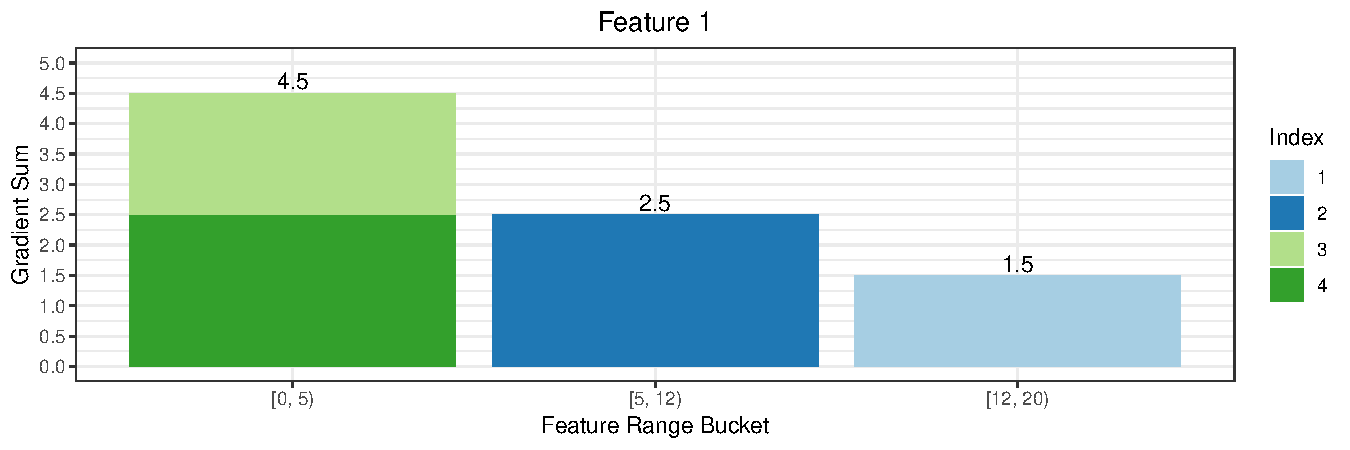
\includegraphics[width=\columnwidth]{feature-one-grad}
	\caption{Gradient histogram for Feature 1 of the Table \ref{tab:example-data} data.
	The first bucket is the sum of the data points with index 3 and 4, since both their Feature 1
	values fall in the $[0, 5)$ bucket.}
	\label{fig:gradient-feature-one}
\end{figure}


The selection of bucket ranges can be done either at the beginning of training, taking the
overall feature CDF, or at every leaf taking the CDF of each feature using only the
partition for that leaf. \citet{xgboost} show that by selecting the buckets for every
leaf separately, we can achieve the same level of accuracy, while using histograms with a higher approximation error, and hence reducing the memory footprint of the algorithm.


Once the bucket ranges have been determined for each feature, we use them to create
the gradient histograms. After the prediction step, we have a gradient value for each data point, so
we go through each feature and add the data point's gradient value to the gradient
histogram bucket
that corresponds to the feature value.
In our example data in Table \ref{tab:example-data}, for Feature 1 we use the
buckets $[0, 5), (5, 12], (12, 20)$.
Then, for the data point $x_1$ with a feature value $f_1 : 13$, we would add its
gradient value to the
the bucket $(12, 20]$ of the gradient histogram for $f_1$, and do this for
every data point, adding the point's gradient to the corresponding bucket given
the feature value. The gradient histogram for Feature 1 is shown in Figure \ref{fig:gradient-feature-one}. In the Figure we use color to identify the
contribution of each data point to each bucket.
When we are done iterating, each feature will have a corresponding gradient histogram,
whose sum is equal to the sum of gradients for the leaf.
For the data of Table \ref{tab:example-data}, the complete gradient histograms
are shown in Figure \ref{fig:gradient-all-features}.

\begin{figure}
	\centering
	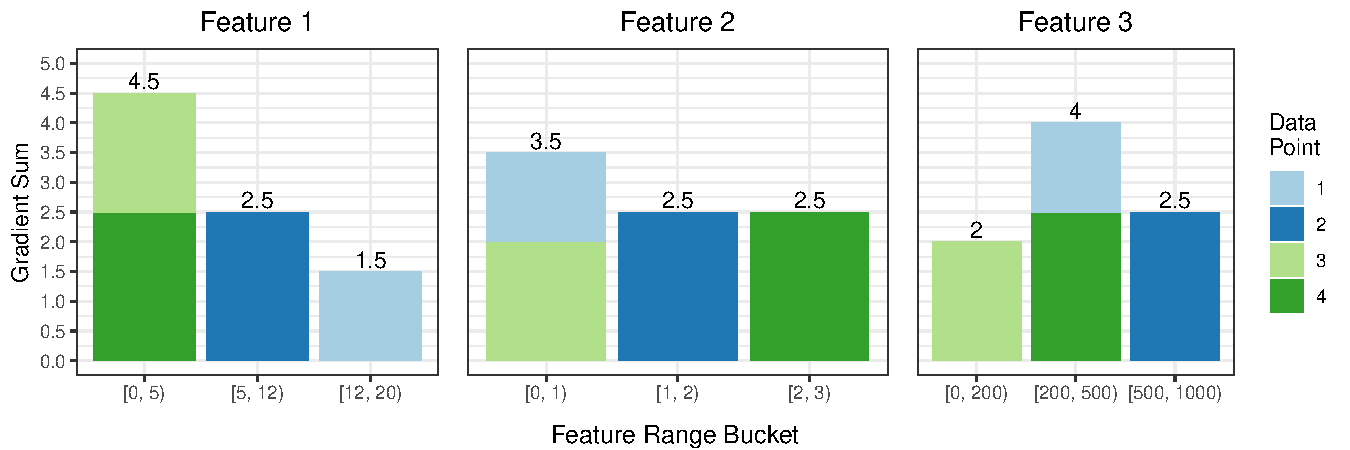
\includegraphics[width=\columnwidth]{all-features-grad-custom}
	\caption{Gradient histograms for all features of the Table \ref{tab:example-data} data.
		}
	\label{fig:gradient-all-features}
\end{figure}

Once we have all the gradient histograms, we can use them to determine the optimal split point for the
leaf, by calculating the potential gain of each feature and split point combination using the following equation~\cite{xgboost}:

\begin{equation}
	\mathcal{G}_{\text{split}} = \frac{1}{2} \left[\frac{\left(\sum_{i \in I_{L}} g_{i} \right)^{2}} {\sum_{i \in I_{L}} h_{i}+ \lambda} + \frac{\left(\sum_{i \in I_{R}} g_{i} \right)^{2}}{\sum_{i \in I_{R}} h_{i} + \lambda} - \frac{\left(\sum_{i \in I}g_{i}\right)^{2}}{\sum_{i \in I}h_{i}+\lambda}\right]-\gamma
\end{equation}

\noindent
where $I_L, I_R$ determine the data points that end up to the left and right side of the split
respectively, $I$ is the complete set of data for the leaf partition, and $\gamma$ a
regularization parameter. At this point, to determine
the best split we need to simply iterate through all the feature-splitpoint combinations
and rank every candidate according to their loss reduction (or \textit{gain}) and select the
best one. In our example we have three buckets, and hence two possible split points for each feature. The result for our example data is shown in Table \ref{tab:gains}, where
we have simplified the problem to only include the first order gradients. From that example
we can see that the best feature-split combination would be choosing the first split
point for the first feature (i.e. Feature 1 $< 5$) as the split condition.

\begin{table}
	\centering
	\begin{tabular}{ccc}
		\toprule
		& Splitpoint 1 & Splitpoint 2 \\
		\midrule
		Feature 1 & \textbf{36} & 21 \\
		Feature 2 & 35 & 30 \\
		Feature 3 & 26 & 30 \\
		\bottomrule
	\end{tabular}
	\caption{Potential gains for each possible split point, given
	the gradient histograms of Figure \ref{fig:gradient-all-features}.}
	\label{tab:gains}
\end{table}

In the case of millions of features and a large bucket count this can also be
computationally heavy operation, as we need to evaluate $|F| \times B$ split candidates.
To mitigate this, we can apply efficient boosting approaches that try
to reduce the number of features being examined. Examples include LazyBoost \cite{lazyboost}
that uniformly subsamples the set of features,
bandit methods \cite{bandits-boosting} that use information from previous iterations, or other adaptive
methods like Laminating \cite{laminating} that determines the best feature in multiple rounds, by incrementally
halving the number of features being considered and doubling the number of examples being
included in the gradient calculations.

\section{Online Decision Trees}
\label{sec:bg-dt-online-trees}

As we have shown, decision trees are trained by recursively splitting the complete
training set as we introduce more leafs. This process is incompatible with the online
learning scenario where data points arrive sequentially and we never have access to
the complete dataset. To tackle such a scenario, a number of online decision tree
alternatives have been proposed.

\subsubsection*{Hoeffding Trees}

By far the most popular online decision algorithm for classification is the Hoeffding Tree (HT) \cite{vfdt},
which has served as the basis for most of the follow up work on online decision
trees. The aim of the HT is to create an online decision tree algorithm that will converge
to its batch equivalent given enough samples.
The learning in an HT, or as \citet{vfdt} name it, the Very Fast Decision
Tree (VFDT), happens only at the leaves, and every data point is only utilized
once, i.e. the HT is a single-pass algorithm. The leaves accumulate statistics
with the purpose of probabilistically determining the best split. The tree gets its
namesake from the use of the Hoeffding bound to determine if we have accumulated
enough information at a leaf to trigger a split with high confidence.

Following the description from \citet{vfdt}, the Hoeffding bound \cite{hoeffding-bound} is a probability inequality that allows
us to probabilistically bound the true mean of a random variable $r$ for which we have
made $n$ independent observations and computed their sample mean, $\bar{r}$. Given
the range of the variable, $R$, the Hoeffding bound states that with probability
$1-\delta$, the true mean of the variable $r$ will be at least $\bar{r}-\epsilon$, where
$\epsilon$ is defined as:

\begin{equation}
	\epsilon = \sqrt{\frac{R^2ln(1/\delta)}{2n}}.
\end{equation}

In VFDT, the Hoeffding bound is used to determine with a high degree of certainty when
it is time to split a leaf. Let $G(X_i)$ be the measure used to choose the feature
to split on. As we mentioned in Section \ref{sec:bg-dt-learning-algorithms}, this can be
information theoretic measures like the cross-entropy or the Gini index. Ideally we want the feature we select given a limited sample of $n$ examples, to be the same as would be chosen given infinite examples.
The Hoeffding bound allows us to achieve that with high probability by applying
it to determine the maximum possible difference between the best and second best
features to split on. Specifically, let $\bar{G}(X_a)$ be the heuristic value for the
current best feature, after having observed $n$ instances, and $\bar{G}(X_b)$ the second
best. The difference between these two is $\Delta \bar{G} = \bar{G}(X_a) - \bar{G}(X_b)$.
We can then use the Hoeffding bound to determine that $\bar{G}(X_a)$ is indeed the
best feature to split on with probability $1-\delta$, if $\Delta \bar{G} > \epsilon$.

The process of learning at each leaf is then the following: For every incoming sample
that ends up in a leaf, we update the sufficient statistics for that leaf, which we
use to calculate the heuristic for the split, e.g. the Gini index. Theoretically,
one could check if we have gathered enough information to split a leaf after each
incoming sample, but that would introduce a large computational overhead. What we
do instead, for example in the implementation of the algorithm in the MOA library \cite{bifet2010moa},
is to only check if the Hoeffding bound is satisfied periodically, for example
every 200 samples. Another parameter of the algorithm is the probability of an error,
$\delta$. This parameter can have a large effect on the final tree, as setting it
too high can lead to early splits being taken that end up being sub-optimal, and as a result,
values in the order of $10^{-7}$ are often used \cite{data-stream-mining}.

HT was designed for the classification setting, where handling discrete attributes
is straightforward: we can just keep a table of frequencies for classes and feature
values. The situation
is different for continuous attributes however, where we need to maintain per-class
information about the values. In the worst case we would need to maintain the class
frequencies for every unique value in a continuous feature, something that is impractical
for online learning, where datasets are potentially unbounded and the memory footprint
of the algorithms should remain as small as possible. For features with many repeated
values it is possible to use a binary tree structure with counters that allows for
fast storage of the values, however this again has a large memory cost. Alternatives include
using online histograms or quantile sketches \cite{greenwald2016quantiles}
to maintain approximations of the Cumulative Distribution Function of
each feature, or approximating the distribution of each continuous feature using a Gaussian.
We refer the interested reader to Chapter 4 of \citet{data-stream-mining} for details on these methods.

The Hoeffding Tree has served as the starting point for most of the follow up work on
online decision trees. \citet{vfdt-normal} use a ``Normal'' test to improve
upon the statistical efficiency of the Hoeffding bound. The proposed method achieves
the same probabilistic bound with a reduced sample size, by taking
advantage of properties of the Gini index and entropy. More recently,
\citet{efdt} propose an algorithm that uses the Hoeffding bounds but
will re-visit nodes that have already been split and evaluate if their
split decision should be updated. This leads to a large improvement in accuracy
compared to the base HT,
at the cost of added computation and memory necessary to maintain
the sufficient statistics for internal nodes and re-evaluate split
decisions.

In a contrasting view, \citet{vfdt-mcdiarmid} claim that the assumptions made
by the Hoeffding bound-based algorithms are commonly violated as the bound assumes
real-valued data, and the fact that measures like the Gini index and information
gain cannot be expressed as sums of elements. As an alternative they propose
using McDiarmid's inequality of which Hoeffding's inequality is a special case.
Their use of the McDiarmid
bound is however computationally intensive. This drawback is mitigated
in their follow-up work \cite{vfdt-gaussian} which follows in part the work from \citet{vfdt-normal}
and provides a bound on the information gain difference between two potential
split attributes based on the Gaussian distribution.

One of the few online decision tree algorithms that is aimed at regression
is the Fast Incremental Model Tree (FIMT) algorithm by \citet{fimt}, also
based on the HT. FIMT
is a model tree, i.e. instead of simply using the average of the labels
in its leaves to make predictions, it maintains a linear model, which is
fit on the samples arriving at the leaf, and is then used for prediction.
The merit of a split is calculated based on the Standard Deviation Reduction (SDR),
similarly to batch regression trees like the M5 model \cite{m5-tree}, defined as:

\begin{equation}
	\begin{split}
		\text{SDR}(h_A)=sd(S)-\frac{|S_L|}{|S|}sd\left(S_{L}\right)-\frac{|S_R|}{|S|}sd\left(S_{R}\right), \\
		sd(S) = \sqrt{\frac{1}{|S|}\left(\sum_{i=1}^{N}y_{i}^{2}-\frac{1}{|S|}\left(\sum_{i=1}^{N}y_{i}\right)^{2}\right)}
	\end{split}
\end{equation}

\noindent
where $h_A$ is the proposed split on feature $A$, and $S_L, S_R$ the resulting
data partitions on the left and right side of the split.

SDR is possible to be calculated online, by maintaining only three statistics per leaf,
making the learning of these trees efficient. However, the base FIMT uses a binary tree
to store feature values, leading to a potentially high memory cost, for which
the authors provide solutions like disabling non-promising split points and dropping
parts of the tree. To determine the
probability of a split being optimal, the authors again use the Hoeffding bound
on the SDR ratio of the two best splits which will be in $[0, 1]$ range.
The linear models at the leaves are perceptron models, updated using stochastic
gradient descent.  Finally, FIMT includes a change detection system in order to
adapt to concept drift
based on the Page-Hinckley change detection test~\cite{ph-test, ph-test2}.

\todo{Online RFs?}

\subsubsection*{Mondrian Forests}

All the methods we mentioned so far have made use of the same base tree building
algorithm that was first proposed for VFDT: each data point is only evaluated once,
the statistics are maintained only at the leafs, with the exception of \cite{efdt},
and heuristics that take into consideration the conditional distribution of the
features given a class are used to determine the splits. \citet{mondrian-forests-original}
proposed a new class of algorithm based on Mondrian processes \cite{mondrian-process}
that provides a new way to train decision trees online.

Mondrian processes are a continuous-time
Markov process that form hierarchical partitions of the feature space $\mathbb{R}^D$.
The partitions are nested and each subsequent partition refines its parent. While
these processes are non-parametric and define infinite partitions, Mondrian trees
restrict them using a \emph{lifetime} parameter $\lambda$.
This parameter is however hard to tune,
so the the authors choose instead to stop splitting nodes when the data points
within them all have the same class value. Compared to regular decision trees,
Mondrian trees have two main differences: The split decisions are always within
the range of observed data, i.e. the split decision create ``boxes'' in feature
space and not axis parallel cuts, and like the Extremely Randomized Tree algorithm
\cite{ert}, the splits positions are chosen uniformly at random. The main property that makes Mondrian trees possible to train
online is \emph{projectivity}. We can grow a new tree by sampling from a restricted
distribution of Mondrian trees that have already been trained, extending the tree
to include the new data. The Mondrian tree distribution is in this sense ``self-consistent''
\cite{mondrian-forests-original} which allows us to grow them from the previously
sampled tree in an online manner. The original Mondrian trees are aimed at classification
and follow up work extends them to handle regression as well \cite{mondrian-forests-regression}.

One main characteristic of Mondrian trees is that they are able to determine the full
predictive posterior distribution of the dependent. This means that they are able to
produce a distribution of the form $p_T(y |\mathbf{x}, \mathcal{D}_{1:N})$, where
$y \in {1,..., K}$ for the multi-class classification scenario, or $y \in \mathbb{R}$
for regression. For classification the posterior is modeled as a hierarchy
normalized stable processes~\cite{nsp}, while for regression a hierarchical Gaussian is used.
The algorithm uses an ensemble of Mondrian trees to create a Mondrian Forest and combine
their predictions for a final output.

The main disadvantage of Mondrian forests is their computational cost. The model
requires that learning happens at all levels of the tree, unlike most of the HT
algorithms where learning only occurs at the leaf level. Because a complicated
model of the posterior needs to be updated, the computational cost of the algorithm
increases with each incoming data point and is $\mathcal{O}(\log n)$ for the $n$'th
data point, or in other words it has a cost of $\mathcal{O}(\log N!)$ to train N
data points. In addition, the online version of the algorithm needs to maintain
all data points at the leafs in order to be able to update the distributions.
This makes its memory cost prohibitive for a streaming setting with limited resources
or unbounded data.

In our work we use Mondrian Forests as the state-of-the-art comparison in \uncertaintrees
and show that we are able to achieve similar accuracy with an order of magnitude reduction
in runtime and bounded computational cost.
\newpage
%\part{Methodology}
%\chapter{Methodology}

\section{Research Strategy}

\section{Evaluating Unsupervised Models}

\section{Evaluating Online Models}

\section{Data Sources}

\section{Ethical Considerations}
%\newpage
\part{Results}
\label{part:results}
\chapter{Graph Vertex Similarity And Concept Discovery}
\label{ch:concepts}
In this chapter we provide a summary of our work on scalable graph similarity calculation.
We describe the problem and some related work in Section \ref{sec:concepts-background}
and describe our approach in Section \ref{sec:concepts-main-findings}. As part of our
results review we present an experiment that was not part of the original work, that
bridges deep learning with out work to extract visual concepts from images.


\section{Background}

\label{sec:concepts-background}

This work tackles the general problem of determining the similarity between \emph{objects}
in a data set, which can take many forms: cosine similarity between
items embedded in a low-dimensional representation \cite{word2vec}, ...
\todo{A second thing here}, or as done
in this work, by modeling the problem as graph similarity calculation.
The use of the generic \emph{object} term here is intentional, as our method is domain-agnostic
and can be applied in a variety of domains where a meaningful measure of correlation
between objects can be derived. In the paper we present examples from the linguistic,
music, and molecular biology domains, and we provide an additional example in this thesis
using images as input, in Section \ref{sec:concepts-openimages}.

In our approach we model the objects as nodes in graph and their interactions as edges,
weighted by a measure of correlation between the objects. In language for example, the
nodes would be words and the edges could be weighted by their mutual information \cite{mutual-information-nlp}.

However, the computation of all-to-all similarities in a graph can quickly become
intractable for large graphs. The popular SimRank algorithm developed by
\citet{simrank} for this purpose,
has a cubic time complexity with respect to the number of nodes in the graph.
Clearly then for large-scale graphs some form of approximation needs to be used
to make the computation feasible.


\section{Method}

We deal with the scalability problem by using a two-step process to calculate similarities.
We first create a \emph{correlation graph} that models the surface correlations between objects.
These correlations are easy to extract and do not necessarily hold semantic information.
For example,
given a corpus of text we can use a
co-occurence measure, like mutual information, between any two pairs of
words and use that as the edge weight between the two in the correlation graph.
We then compute the similarities between nodes by applying a transformation on this graph, to produce a graph which surfaces deeper,
semantic interactions which we term the \emph{similarity graph}.
In order to determine the similarity between objects in graph, we examine
their agreement in correlations to other objects: if two nodes are highly
correlated to similar sets of nodes, they are more likely to be similar themselves.

However, computing these all-to-all similarities can be challenging for massive
correlation graphs.
As in other works in this thesis, we apply a combination of using approximations to limit
the computational cost of the method, and develop a distributed algorithm that allows
us to scale-out learning and take advantage of modern computing clusters.

The first approximation we employ makes use a characteristic that many real-world datasets exhibit,
that is, there exists a long-tail distribution of interactions between items in a graph. These type
of ``small-world'' graphs, appear in areas like gene co-expression \cite{gene-small-world}, semantic networks \cite{semantic-small-world},
word co-occurrences \cite{words-small-world} and social networks (see \cite{barabasi-small-world} for further
examples).
This allows us to prune the input correlation graph significantly before transforming it,
while maintaining a controllable and small approximation error.

The second approximation has to do with the locality of the computation. Instead of trying
to solve the computationally intractable all-to-all similarity problem, we instead only look at
nodes that are one hop apart, keeping the computation local and dramatically limiting the number of
cost per node in the graph.
This approximation is what makes the distributed implementation of the algorithm efficient.
In order to compute for each pair of nodes in a neighborhood their common sets of correlated nodes,
we need only examine the common sets of incoming edges per node. By distributing our graph
using the id of the incoming nodes as a key we can perform this computation using a
self-join operation, which involves no communication of data in the cluster. As a result
we are able to scale the computation to massive datasets, as we demonstrate with our use of the
Google Books n-gram dataset, which corresponds to approximate 4\% of all the books ever
printed \cite{ngrams} (24.5 billion rows).

Once we have built the similarity graph, we can go one step further in order to extract
groups of inter-similar objects that we call \emph{concepts}. These correspond to groups
of objects that belong to the same semantic group, based on their appearances in the context
of other objects. In the language example these could be words that describe the same
concept such as ``cities'', or words with the same syntactic and semantic purpose, like
groups of adverbs. To create these groups we apply a community detection method on top
of the similarity graph. Because the similarity graph itself can be large, we develop
a scalable approach which is based on the speaker-listener label propagation algorithm
(SLPA) \cite{slpa}. \todo{Do we explain community detection and label propagation here?}

\section{Main Findings}

\label{sec:concepts-main-findings}

In the paper we provide examples of the output produced by the algorithm, and
perform an evaluation of the similarities produced using a gold standard dataset,
WordSim-353~\cite{wordsim}. Here we provide a summary of some of the experiments
presented in the paper, and a new set of results using images as input.

\subsection{Billion words corpus}

In the paper we perform an evaluation on the Billion word corpus~\cite{billion-word}
which contains approximately one billion tokens and was scraped from online news
sources. We create the correlation graph by using the relative co-occurrence frequency
of word pairs, that is the (directed) correlation between the words $i$ and $j$, $\rho_{i, j}$,
will be $c_{i,j}/c_i$ where $c_{i,j}$ the number of times the words co-occur within
a window, and $c_i$ the frequency of word $i$ in the corpus. For this experiment we
select a window size of two, meaning we only take into account bigrams.
We can some example concepts uncovered by the algorithm in Figure \ref{fig:concepts-billion}.

\begin{figure}
	\centering
	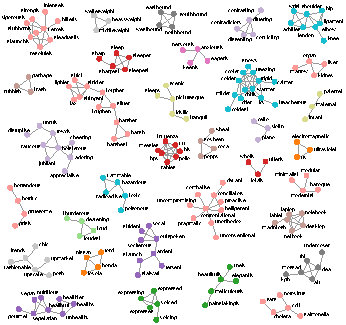
\includegraphics[width=\textwidth]{billion-words-example}
	\caption{Example concepts extracted from the Billion word corpus}
	\label{fig:concepts-billion}
\end{figure}

\subsection{Music}

We also perform experiments on a music listening dataset created by Celma from
the Last.fm music service~\cite{celma-long-tail}. The dataset contains 19 million
track play from 992 users, which we use to create a correlation graph between
artists. The correlation measure $\rho_{i, j}$ is the number of times artist $i$ was followed
by artist $j$, divided by the total number of plays for artist $i$. Some example
artist concepts which correspond to the music genres can be seen in Figure
\ref{fig:concepts-artists}.

\begin{figure}
	\centering
	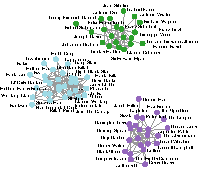
\includegraphics[width=0.8\textwidth]{artist-example}
	\caption{Example concepts extracted from the music listening dataset.}
	\label{fig:concepts-artists}
\end{figure}

\subsection{Visual concepts through the combination of Deep Learning and graphs}

\label{sec:concepts-openimages}

In this experiment we make use of a combination of deep neural networks and our
algorithm to uncover visual concepts from raw images. Deep neural networks
can be trained on labeled datasets of images to recognize multiple objects
in an image \cite{deep-learning}. The networks' accuracy creates a unique opportunity
to generate visual concepts out of raw images: A network trained on labeled dataset
like ImageNet \cite{imagenet} can be used to generate labels from unlabeled raw images thus generating
a ``silver-standard'' dataset which we can use as input for our algorithm.

In our experiments we have used the OpenImages dataset \cite{openimages} which uses
multiple image classifiers to annotate images with labels from 19,794 different
classes. The complete training
dataset contains 9,011,219 images scraped from the Flickr service\footnote{\url{www.flickr.com}}, of complex scenes annotated with 8.4 objects per image on average.

We use the OpenImages data to create a correlation graph of objects: We form
a clique for every object that exists together in one image, creating a graph that represents
how objects commonly appear together in real images. Take for example the annotated
image shown in Figure \ref{fig:horse-hat}. The image is annotated with both the
\emph{horse} and \emph{cowboy hat} labels. All the labels in the image will form
a clique in our graph. Looking at another image, \ref{fig:hat-guitar} we can now
extend this graph, by connecting the \emph{cowboy hat} label with the \emph{guitar}
label, creating a second degree link between the \emph{horse} and \emph{guitar} labels.
By incorporating all such images, our correlation graph will have a representation of objects
that tend to appear together in the real world. Using this graph as input, we can apply our similarity
transformation to group together objects that belong to semantically similar classes
based on the similarity between the contexts in which they appear in, in the real world.
Finally we can apply our community detection algorithm to group together items to form
visual concepts in the similarity graph.

To illustrate the uncovered concepts, we take the 30,000 most similar
pair-wise object similarities and present the output similarity graph in Figure \ref{fig:openimages-concepts}, where the colors indicate the uncovered concepts.
To ease presentation we provide two zoomed-in parts in Figure \ref{fig:openimage-zoom},
where we can see objects that can roughly be described as ``uniformed people'' are grouped
together in Figure \ref{fig:openimages-military}, and objects that relate to cameras
grouped together in Figure \ref{fig:openimages-cameras}.

Using our algorithm in combination with deep learning models, we can use the wealth of unlabeled
images that exist in services like Flickr to create visual concepts.

\begin{figure}
	\centering
	\begin{subfigure}{\textwidth}
		\centering
		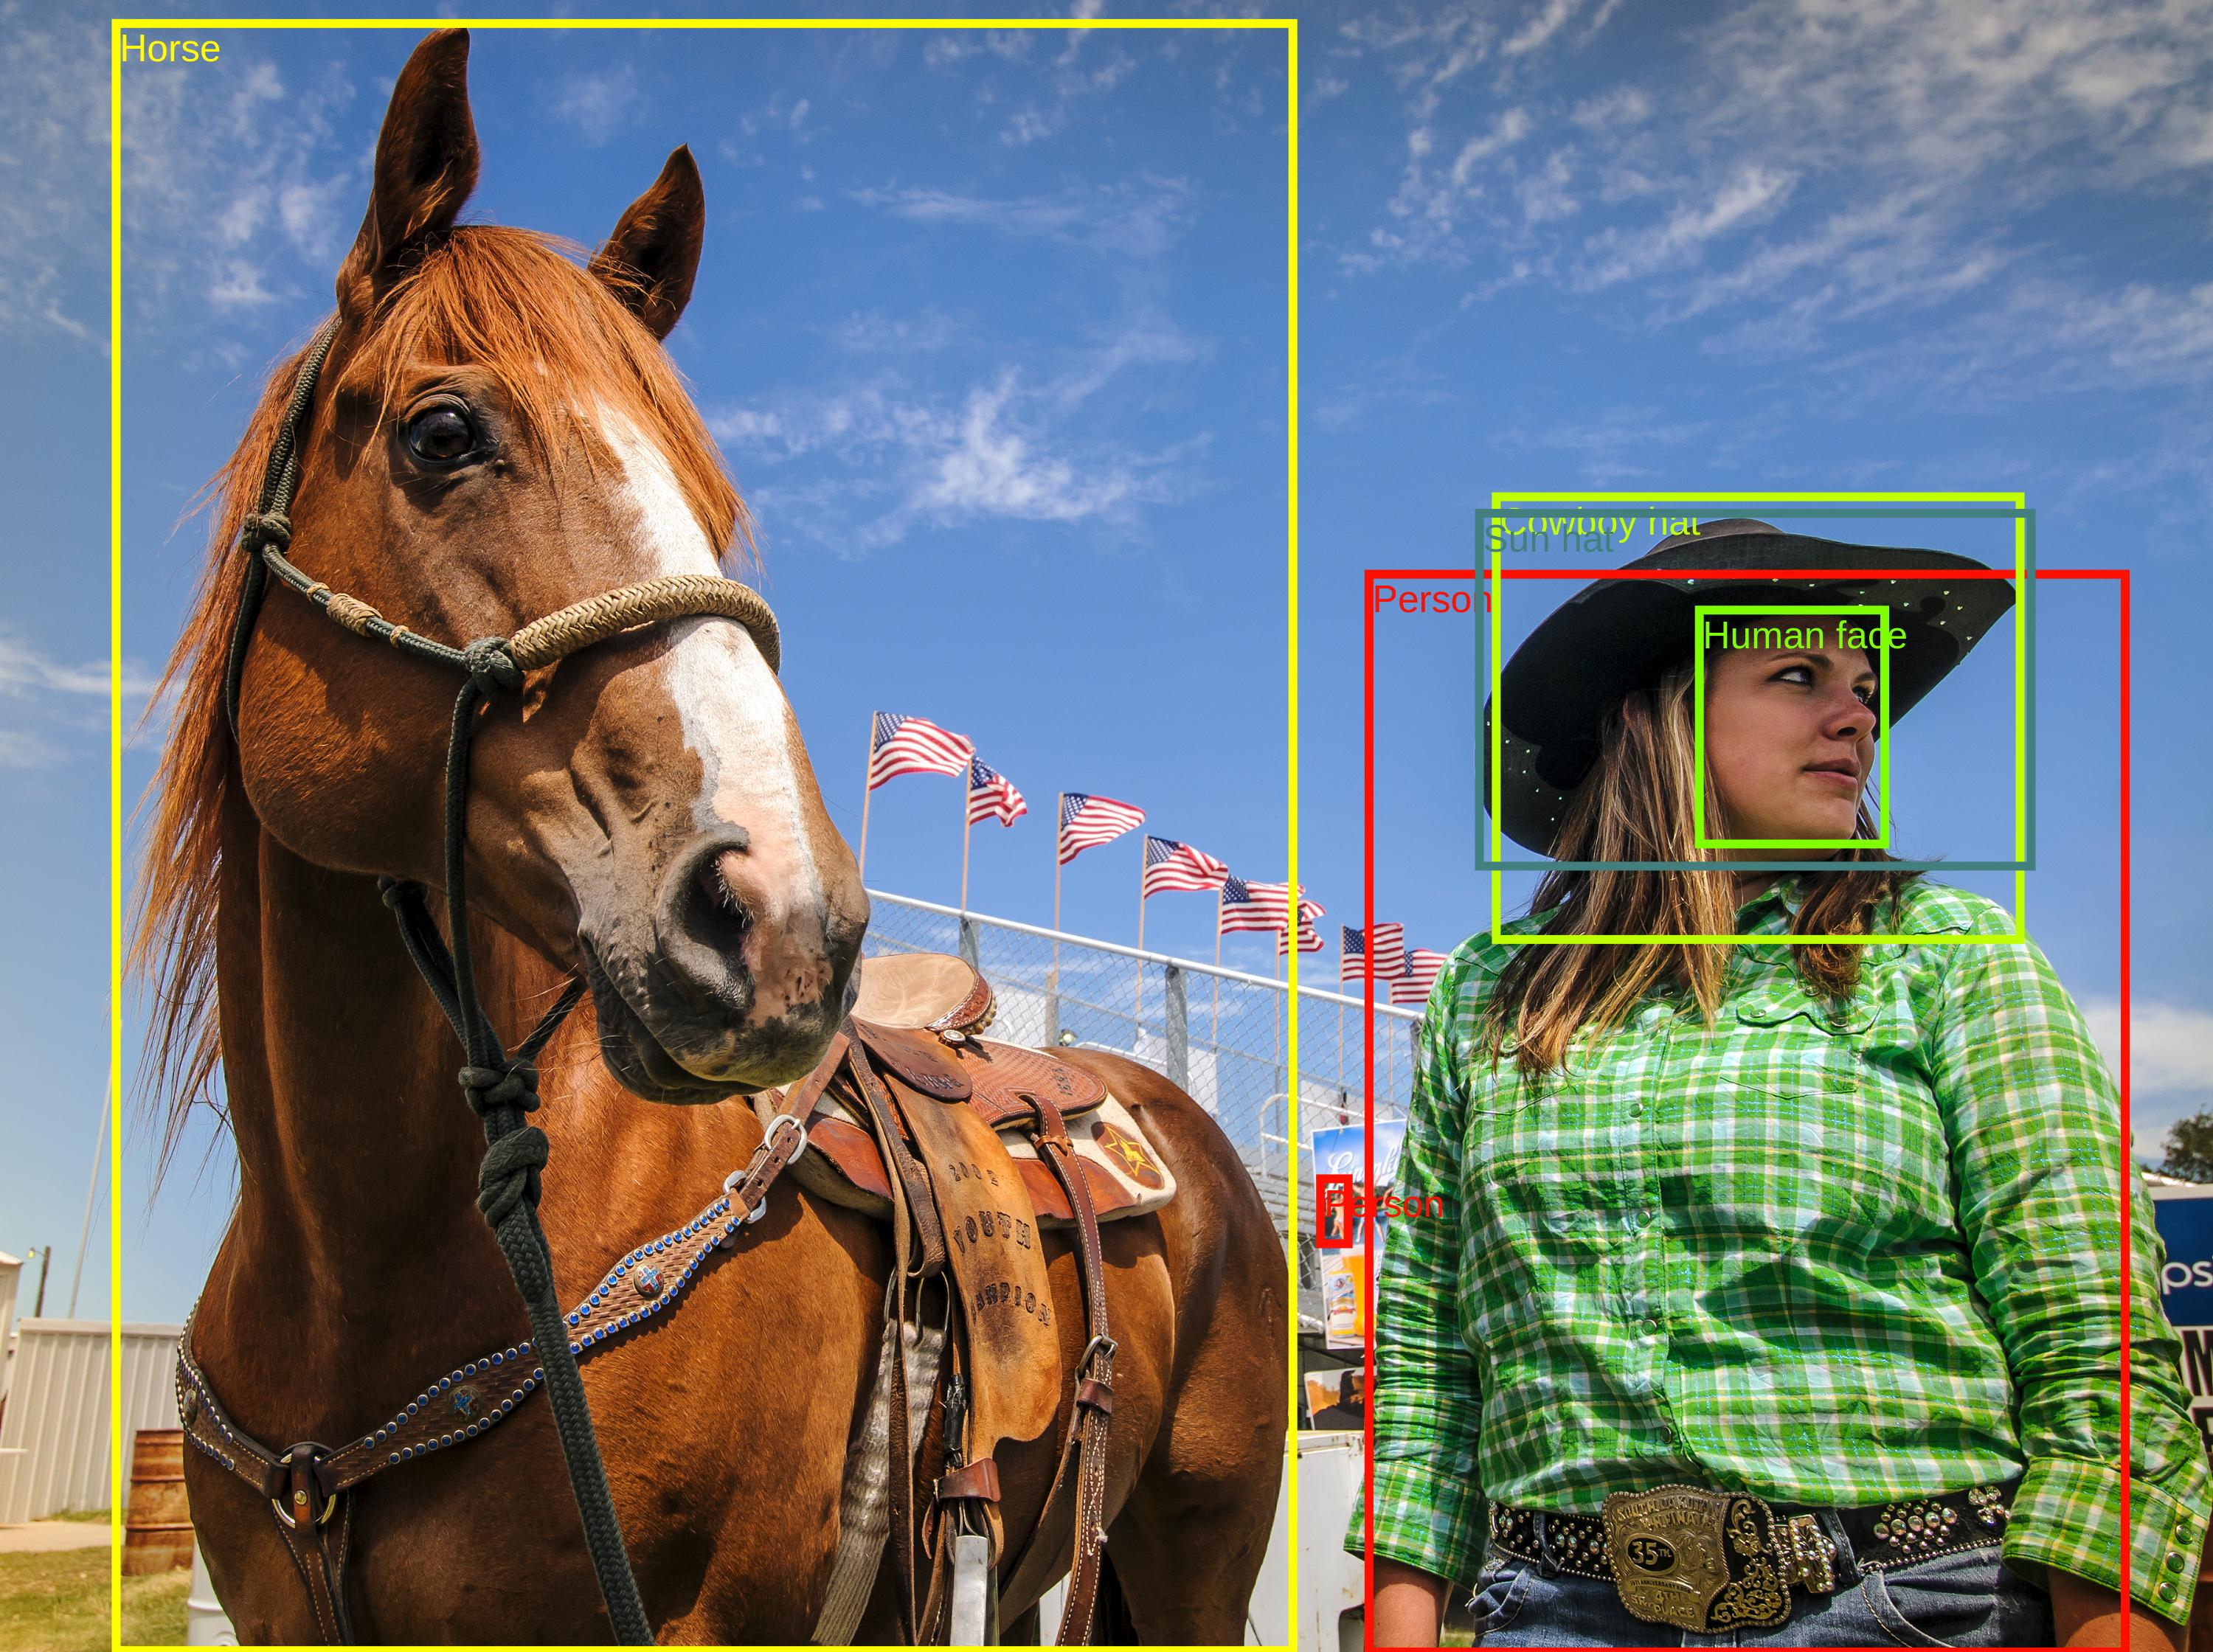
\includegraphics[width=0.9\textwidth]{horse-hat}
		\caption{An image that contains a horse and a cowboy hat.}
		\label{fig:horse-hat}
	\end{subfigure}
	~ %add desired spacing between images, e. g. ~, \quad, \qquad, \hfill etc.
	%(or a blank line to force the subfigure onto a new line)
	\begin{subfigure}{\textwidth}
		\centering
		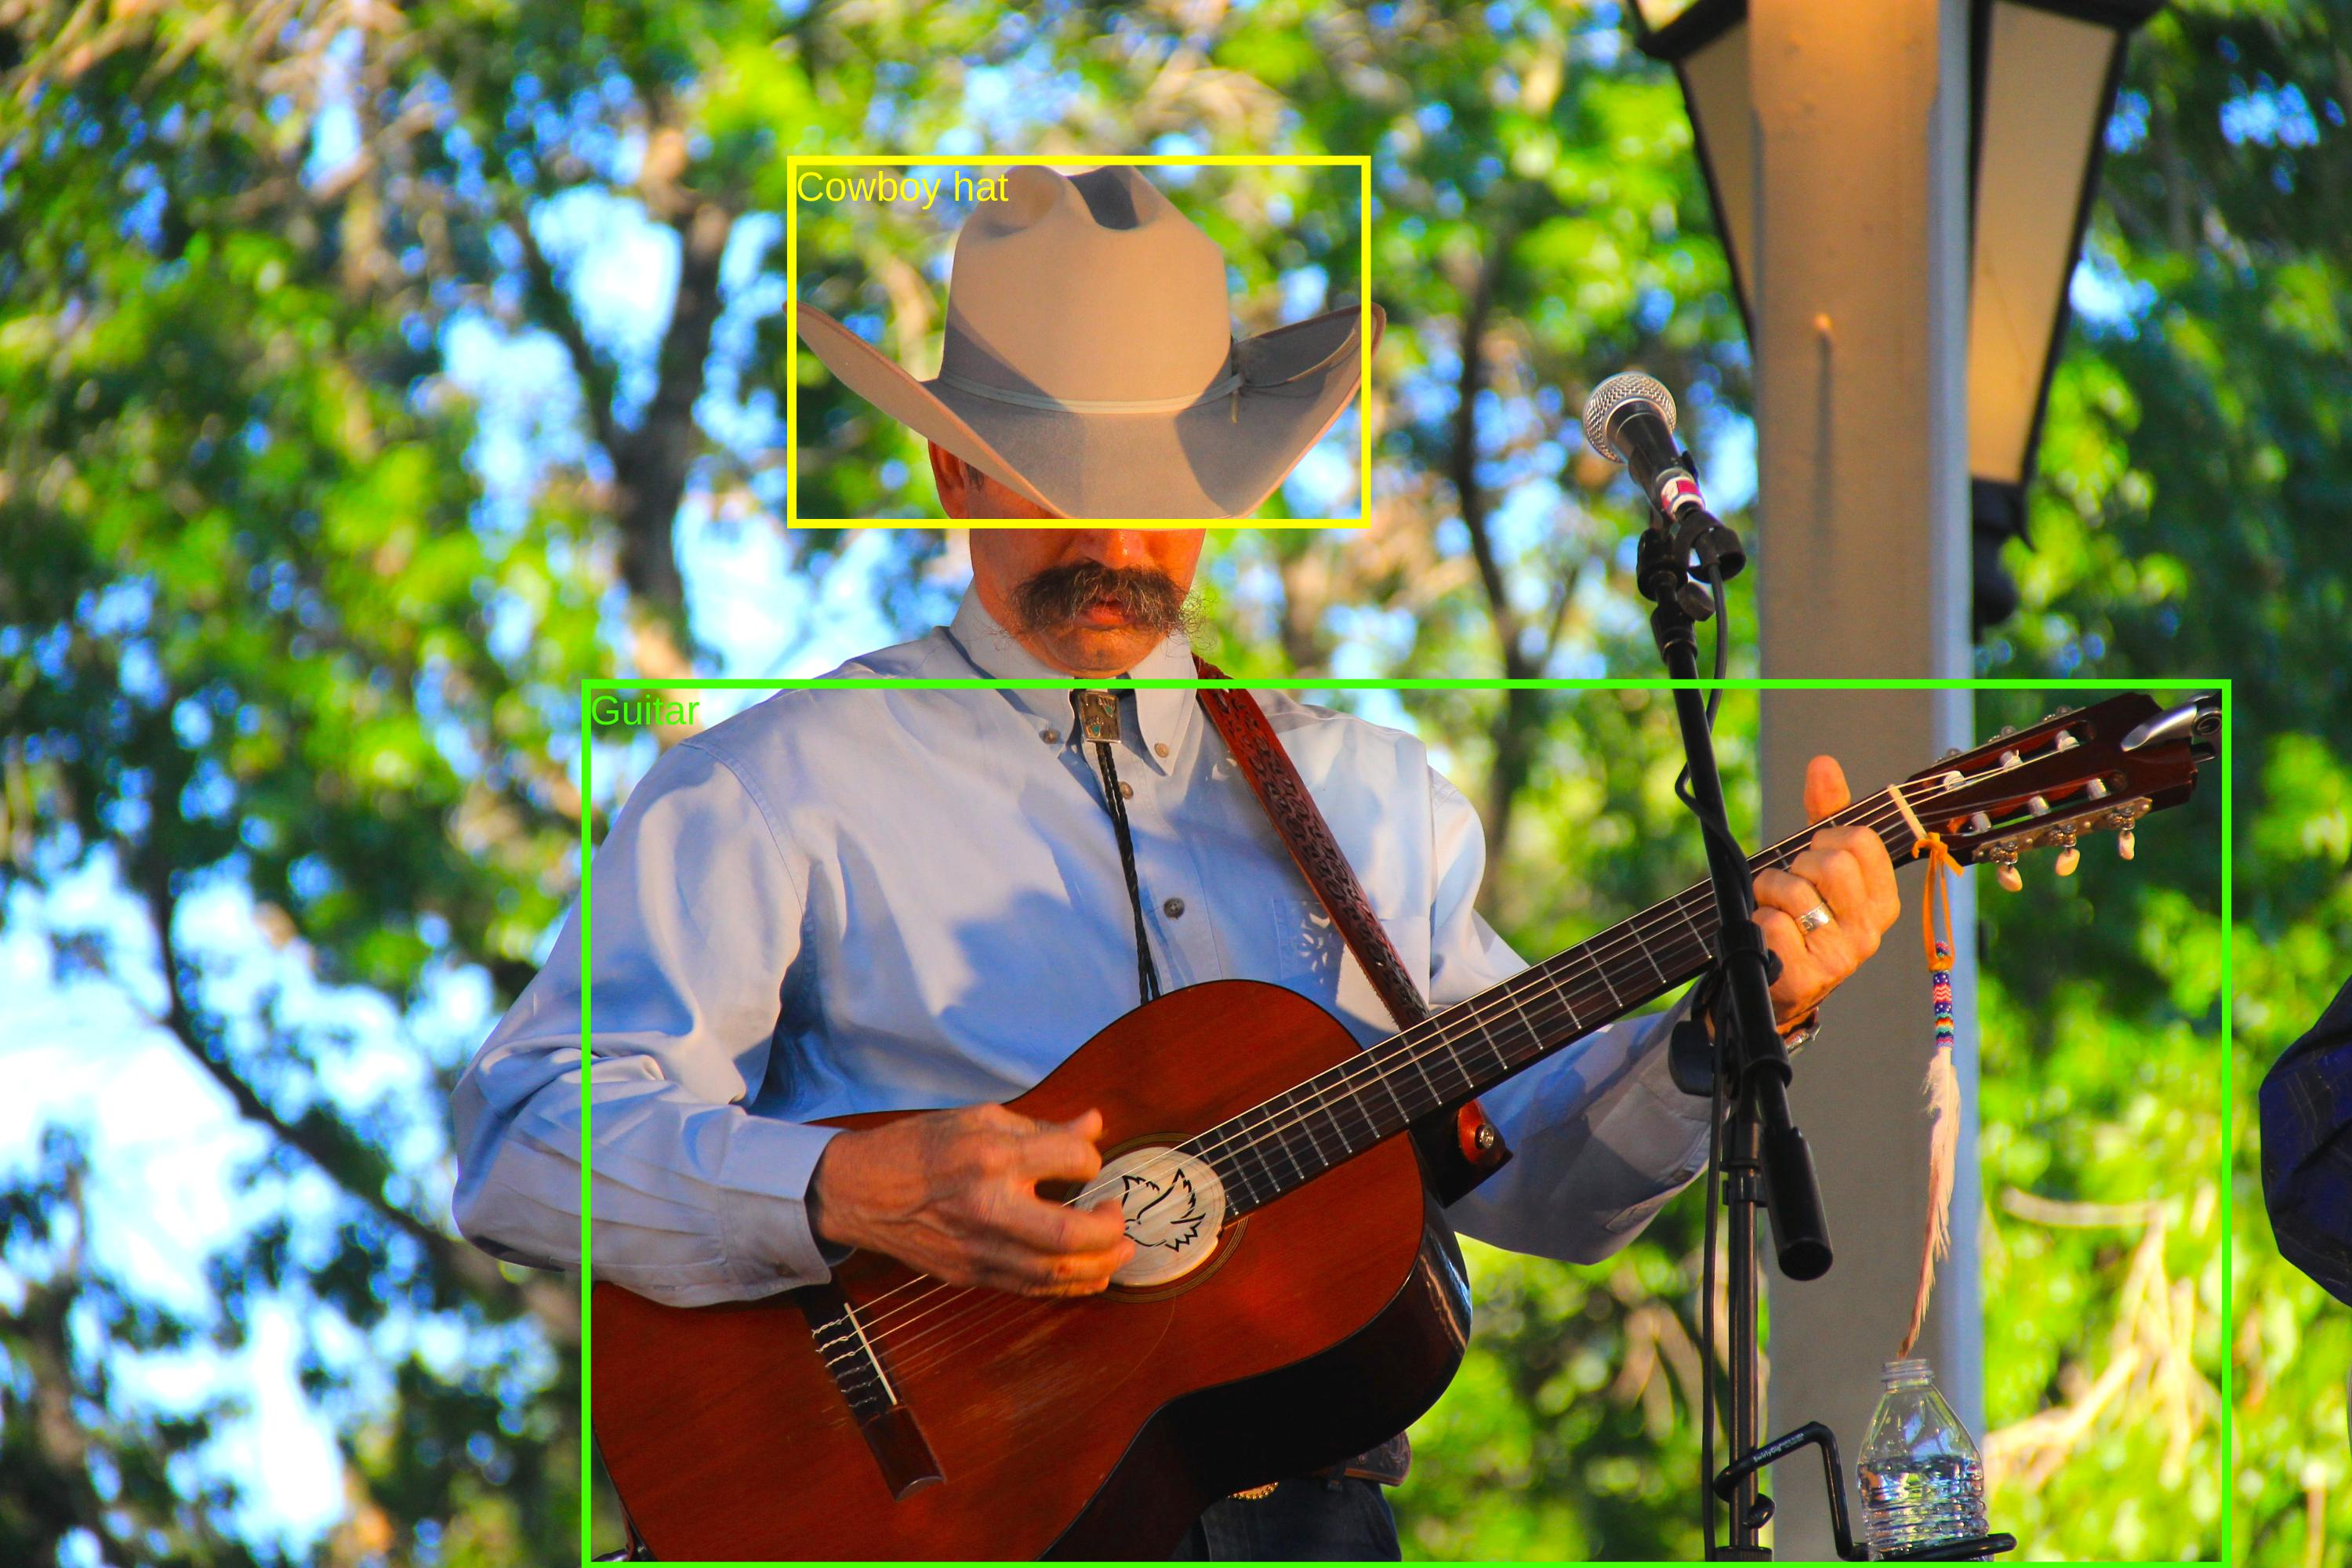
\includegraphics[width=0.9\textwidth]{hat-guitar}
		\caption{An image that contains a cowboy hat and a guitar.}
		\label{fig:hat-guitar}
	\end{subfigure}
	\caption{Examples of annotated images from the OpenImages dataset.}
	\label{fig:openimage-examples}
\end{figure}

\begin{figure}
	\centering
	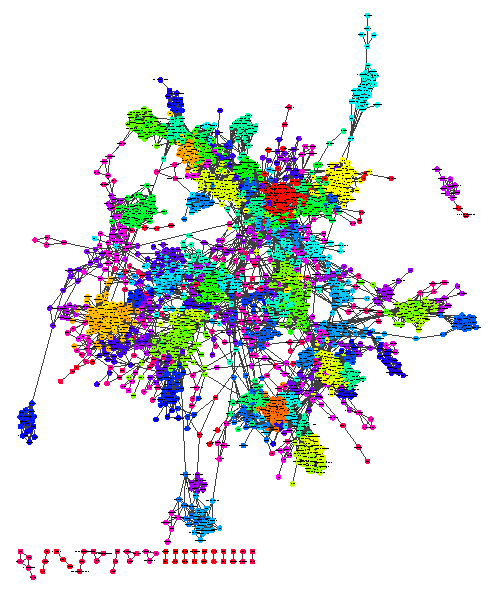
\includegraphics[width=\textwidth]{openimage-communities}
	\caption{The concepts uncovered by using the OpenImages data as input to our algorithm.
	The labels are legible through zooming in the electronic version. See Figure \ref{fig:openimage-zoom} for zoomed-in crops of the graph.}
	\label{fig:openimages-concepts}
\end{figure}


\begin{figure}
	\centering
	\begin{subfigure}{\textwidth}
		\centering
		
\includegraphics[height=0.44\textheight]{openimage-communities-military}
		\caption{A concept that brings together uniformed people and military objects.}
		\label{fig:openimages-military}
	\end{subfigure}
	 %add desired spacing between images, e. g. ~, \quad, \qquad, \hfill etc.
	%(or a blank line to force the subfigure onto a new line)
	\begin{subfigure}{\textwidth}
		\centering
		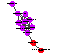
\includegraphics[height=0.44\textheight]{openimage-communities-cameras}
		\caption{A concept that groups together camera equipment.}
		\label{fig:openimages-cameras}
	\end{subfigure}
	\caption{Two visual concepts from the top-right corner of
		Figure \ref{fig:openimages-concepts}.}
	\label{fig:openimage-zoom}
\end{figure}

\subsection{Word similarity evaluation}

To provide a quantitative evaluation of the method we made use of the WordSim-353 (WS-353)
dataset. This dataset includes 353 word pairs that are rated by humans for their
similarity. This dataset includes unrelated words which presents a problem for
approach that by design does not calculate similarities for words that are unrelated,
as using the graph structure is one of the main ways we can make the computation
scale. For that reason we use the word pairs that appear both in the evaluation
dataset \textit{and} exist in our similarity graph. We use the Google n-grams
data with a corpus of 361 billion tokes, which in under 10 minutes produces
a similarity graph that contains 60\% of the word pairs present in WS-353.

The produced similarities have a Spearman rank correlation of 0.76, which
is exactly what the inter-annotator agreement is for this dataset.
Finally we compare the WS-353 and our produced similarities with the
cosine similarities of the GloVe~\cite{glove} embedding vectors,
which was at the time of publication the state of the art embedding
method. We train our method on a smaller corpus and smaller window than
the GloVe vectors, but are still able to generate similarities comparable
to GloVe (0.71 Spearman rank correlation)
\newpage
\chapter{Use-case: Session Length Prediction}
\label{ch:session-length}
In this chapter we provide a real-world use-case that serves as motivation 
for the rest of the work described in this dissertation. After giving
an introduction to the problem and related work in Section \ref{sec:session-length-background},
we describe the methods we used to analyze the data and make predictions in
Section \ref{sec:session-length-method} and summarize our findings in Section
\ref{sec:session-length-main-findings}. Finally, we provide desiderata
for a real-world system and identify gaps in the current state-of-the-art
research. We provide solutions to each of the
specific problems identified here in the following chapters.

\section{Background}
\label{sec:session-length-background}

As media streaming services have proliferated it has become important for streaming
companies to analyze their users' behavior to optimize their offering and
meet their business goals. One important factor in user satisfaction is the length of
users' sessions~\cite{dwell-time-satisfaction}, which we define as the
the complete interaction of a
user starting up the service, consuming a number of items, and ending
their interaction after some elapsed time.
This kind of interaction has been studied in the web search \cite{dwell-time-satisfaction, search-time-model} and ad click \cite{post-click-ads, post-click-survival}
domains, but no study had investigate the media streaming domain before.

Streaming services can use the length of user session to optimize their
recommendations, for example providing exploratory and more ``risky'' recommendations
for long session, versus exploitation and more ``safe'' recommendations for short sessions.
In ad-supported services, having an indication of the session length can also help
with scheduling ads, allowing the provider to hit their revenue target, while
minimizing the annoyance to the user~\cite{annoying-ads}.

Predicting the length of user sessions in a mobile streaming service can be challenging,
because user interaction lengths
typically exhibit long-tail distributions \cite{post-click-survival, weibull-web-browsing, phonecalls}, and the number of external factors that can influence the length of the
session can be hard to model, like users commuting, taking phone calls, or connectivity
issues. Media streaming sessions also differ from dwell time after ad clicks
and web search. In music specifically, which is the domain we are examining,
users typically consume multiple items in one session and have different behaviors
depending on the type of session as we show in our results (Section \ref{sec:session-length-main-findings}).

In our paper we provide an analysis the session length distribution using
tools from survival analysis and use gradient boosted trees with specialized
loss functions to place the probability mass correctly.

\section{Analysis and Prediction of Media Streaming Session Length}
\label{sec:session-length-method}

In this section we describe the methods we have used to analyze the data
and create a predictive model for session length.

\subsection{Weibull Analysis of Session Length}

To analyze the user length behavior of the users we use tools from survival analysis~\cite{survival-analysis}, and specifically the Weibull distribution
\cite{weibull-survival}. The Weibull distribution is a flexible parametric distribution,
commonly used in survival analysis because it allows to model different kinds of failure
rates, where the probability of a unit failing changes over time. Its probability
density function is:

\begin{equation}
\label{eq:weibull-pdf}
f(t) = \frac{k}{\lambda}\left( \frac{t}{\lambda}\right)^{k-1}e^{-(t/\lambda)^k}, t \geq 0
\end{equation}



that provides two parameters: the shape $k$ and the scale $\lambda$. The shape $k$ determines
the evolution of the failure rate over time, while the scale, $\lambda$, determines the spread
of the distribution. The effect of $k$ is best shown through an illustration of the hazard rate
for the Weibull function, that gives us the failure rate for an item that has survived until time
$t$:

\begin{figure}
	\centering
	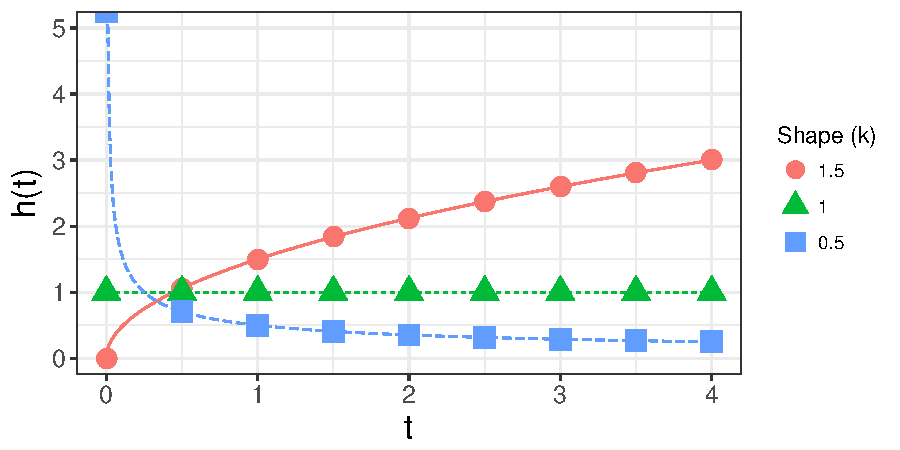
\includegraphics[width=0.7\textwidth]{weibull-hazard}
	\caption{The failure rate of the Weibull distribution for different values of the shape parameter, $k$. We set $\lambda = 1$.}
	\label{fig:weibull-failure-rate}
\end{figure}

The failure rate increases with time for $k > 1.0$, which is called the ``positive-aging''
effect, and decreases with time for $k < 1.0$ an effect called ``negative-aging''. Positive aging
is what we commonly associate with web sessions and is indeed observed in 98.5\% of post-click
behavior\cite{weibull-web-browsing}: as time goes on users become more likely to quit the session
at any point. On the other hand, negative aging means that sessions become less likely to end
as time goes on. This behavior is also described as ``infant mortality'' where defective units
may fail early on, but as time goes on they become less likely to fail.
For $k = 1$ the failure rate is constant and the distribution becomes equivalent to the
exponential distribution.

\subsection{Prediction}

On the prediction side, in order to tackle the issue of the long-tail distribution
of the sessions and to extract as much power as possible from the predictive features,
we choose the gradient boosted tree (GBT) algorithm. GBTs allow us to customize the
loss function to better fit the long-tail distribution of the dependent, and are flexible
enough to discover patterns in the large data we have available.

We extracted a set of features for each user, like their gender, age, subscription
status (pair or free user), and a set of contextual features each session,
like the device type the session is on, the type of network (mobile, WiFi), or
the duration of the last session.

Using these features we train a Gradient Boosted Tree model. We choose this model
because it allows for native handling of missing data which are present in our
data, a common issue in industrial datasets, and for its flexibility in terms of
loss function.

Our data are non-negative and long-tail distributed. One common solution in
these cases is to log-transform the dependent and then fit using a squared
loss, but we often want to use a loss function that is better suited to the
objective. To that end we try fitting both on the log-transformed data with
a mean squared error objective, as well as fitting on a log-likelihood
objective of a Gamma function with a log link function, which can explicitly
model non-negative data with a positive skew. We also test two versions
of each model: One where all data are aggregated and we build a single model,
and one where we build a personalized model for each user.


\section{Main Findings}
\label{sec:session-length-main-findings}

\subsection{User session distribution characteristics}

We use a dataset of user interaction from the Pandora music streaming service, which
is a major US-based music streaming service, and mainly ad supported. We define
sessions as periods of listening activity that are demarcated by breaks or pauses of
30 minutes or more.
We gather data from a random subset users for the months of February to April 2016,
resulting in 4,030,755 sessions. We plot the normalized duration data in Figure
\ref{fig:session-length-times}.


\begin{figure}
	\centering
	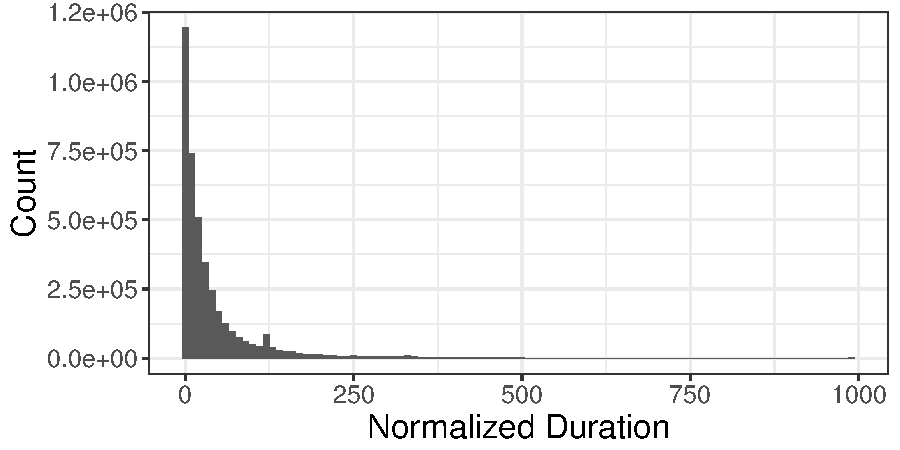
\includegraphics[width=0.7\textwidth]{duration-hist}
	\caption{Histogram plot of session length. The x-axis has been normalized to the 1-1000 range.}
	\label{fig:session-length-times}
\end{figure}

We analyze the session length distribution by fitting a Weibull distribution
to each user's data, and plot the resulting Empirical Cumulative Distribution
Function for the shape parameter in Figure \ref{fig:session-length-shapes}.
We can see that unlike the web site visits after a search, that had a negative aging
effect ($k < 1$) for 98.5\% of the users, only 44\% of the users exhibit the
this behavior for music streaming. The behavior of the users is then split
roughly down the middle, with some users having sessions that become more likely
to end as time goes on, and others whose sessions become less likely to end as
they grow longer.


\begin{figure}
	\centering
	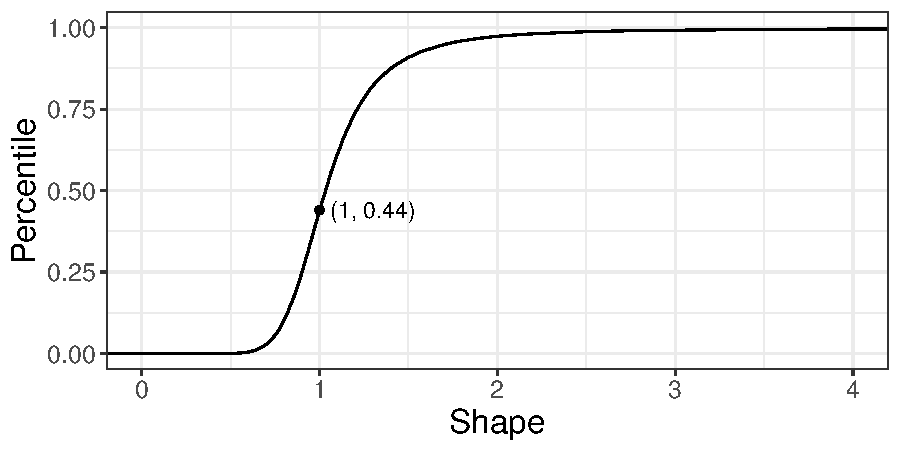
\includegraphics[width=0.7\textwidth]{weibull_shape_ecdf}
	\caption{The empirical cumulative distribution for the shape parameter per user.
		The x axis has been truncated at $x=4$ for readability (~99.5 \% of data points shown).}
	\label{fig:session-length-shapes}
\end{figure}

\subsection{Predictive model performance}

In our analysis of the performance of the predictive model we use two metrics:
First, we use the normalized Root Mean Squared Error which is a common choice
for regression problems, and the normalized mean absolute error, a metric that is robust to outliers, to account
for the long-tail distribution of the dependent. For a baseline predictor we use the mean
session length, a heuristic that is simple, but personalized.
We present the results in Table
\ref{tab:session-length-prediction}.


\begin{table}
	\centering
	\caption{Performance metrics for length prediction task. We report the
		mean value across the 10 CV folds, and the standard deviation in parentheses.}
	\label{tab:session-length-prediction}
	\begin{tabular}{lll}
		\toprule
		Method (\textit{Objective}) & Normalized MAE & nRMSE \\
		\midrule
		Baseline & 1 \textit{(0.001)} & 1.16 \textit{(0.005)} \\
		Aggregated (\textit{MSE}) & \textbf{0.71} \textit{(0.008)} & 1.23 \textit{(0.008)} \\
		Aggregated (\textit{Gamma}) & 0.93 \textit{(0.007)} & \textbf{1.10} \textit{(0.005)} \\
		Per-user (\textit{MSE}) & 0.83 \textit{(0.002)} & 1.29 \textit{(0.004)} \\
		Per-user (\textit{Gamma}) & 0.86 \textit{(0.001)} & 1.31 \textit{(0.003)} \\
		\bottomrule
	\end{tabular}
\end{table}

From the results we can see that the aggregated models perform better overall,
something that can be explained by the fact that the per-user models are trained
on a few data points for most users, leading to over-fitting. The models using the
MSE objective place most of their probability mass closer to the origin and as a
result perform better in terms of MAE, but miss many of the longer sessions
and as a result perform worse in terms of RMSE.

\section{Discussion}
\label{sec:session-length-limitations}

In this Chapter we presented our work on the analysis of session
length distribution in media streaming, and presented a specialized
predictive model.
Through this work we are able to identify several limitations in the current
state of the art in decision tree learning.

First, this work demonstrated the need for algorithms that are
able to learn online and adapt to a constantly changing environment. When
providing estimates of users' session length, we want the predictions of
the algorithms to adapt to the patterns exhibited throughout the day, 
such as day/night and work/home cycles, and be able to adjust to drifting
distributions. 
In order to be able to continuously adapt our models, we have focused on online learning
methods in Papers \boostvhtNum and \uncertaintreesNum that are both scalable and can continuously update tree models with new information about the world.

Second, we were able to identify the importance of quantifying the uncertainty
in predictions. For a quantity such as session length, exact predictions can
be of little value.
The ability to quantify the uncertainty in a prediction can be more useful as
it allows us to make decisions with confidence and avoid giving users
a bad experience. 
For example, if we know with a high degree of certainty
that the true value of the session length will be between 30 and 45 minutes
we can optimize recommendations and ad scheduling for a long running session.
While there exist methods that are able to provide uncertainty estimates
from decision trees for static datasets, no methods exist for online decision trees.
\uncertaintrees
fills this gap in research that combines an online learning model
with the ability to provide uncertainty estimates.

Finally, during this study we were able to get first hand experience with
the accuracy, flexibility and scalability that boosted decision trees
provide. The success of boosted trees has been well-documented,
from winning data mining competitions \cite{xgboost}, to being the model of choice for mission-critical
applications such as ad targeting at major enterprises \cite{mcrank, ctr-facebook}.
What's common in these applications is the need to deal with potentially very
high-dimensional data at scale.
In our follow-up work, we have focused on expanding the 
area of scalable boosted trees for high-dimensional data in Papers \boostvhtNum in the online
domain, and \blockgbtNum in the batch domain.
\newpage
\chapter{Uncertainty Quantification In Online Decision Trees}
\label{ch:uncertain-trees}
In this chapter we present our work on estimating the uncertainty
in the predictions of online decision trees. We define the problem
and present some related work in Section \ref{sec:uncertain-trees-background},
describe the two algorithms developed for this purpose in Section
\ref{sec:uncertain-trees-method} and present our empirical evaluation
results in Section \ref{sec:uncertain-trees-results}.
We close the chapter with a discussion placing the work in the
context of our original research question in Section \ref{sec:uncertain-trees-discussion}.

\section{Background}
\label{sec:uncertain-trees-background}

As machine learning methods mature and become increasingly popular, they are more
often being deployed in critical scenarios were mistakes can be costly. Such
domains include autonomous vehicles, and the medical and financial sector.
In order for critical decision-making to be done by learning algorithms in these areas, we need
to have a notion uncertainty in the algorithms' predictions.
Some of these critical domains also include the requirement that critical decisions
be made in real-time in a constantly evolving environment, and under a tight computational budget. Examples include the financial domain \cite{streaming-finance} and autonomous vehicles \cite{av-safety}.

These examples demonstrate the need for highly accurate algorithms that can be trained
online, adapt to an evolving environment, and quantify the uncertainty in their
predictions. Most of the online learning methods available today do not offer
quantification in their predictions, while most methods that provide uncertainty
estimates are designed for the batch domain where the data are static and bounded.
In this work we aim to provide highly accurate algorithms that can be trained
online, on a sequentially arriving and potentially unbounded dataset, that also
provide uncertainty estimates for their predictions.

We develop two algorithms, one based on conformal prediction~\cite{vovk2005algorithmic} and one based on quantile
regression forests~\cite{meinshausen2006quantile}. The two algorithms are general random forest learners that
enable high accuracy \cite{hundreds-classifiers}, are computationally bounded
and adapt to concept drift through the use of online base learners \cite{fimt},
and provide uncertainty estimates at an accuracy level equal to or better
than the state of the art \cite{mondrian-forests-original}, while being an order of magnitude faster to run.

\section{Uncertainty Estimation for Ensembles of Online Decision Trees}
\label{sec:uncertain-trees-method}

In this section we provide an overview of the methods developed for this work.
We provide a brief description of the batch algorithms that we base our algorithms
on, and proceed to explain how we make use of approximations to transfer them to
the online domain. We deal with the regression task, and our task is to develop algorithms
that exhibit what is called \emph{conservative validity} in conformal prediction literature. This refers
to algorithms that produce predictive intervals such that the probability of the true value not
being part of the interval is \emph{less than or equal to} $\alpha$, which is referred
to as the \emph{significance level}. This task is different from quantile regression \cite{koenker2005qr}
where the objective is for the error level to be \emph{exactly} $\alpha$.

\subsection{Inductive Conformal Prediction}

Conformal prediction (CP) is a meta-algorithm that can add the ability to
produce \emph{prediction regions}, that is, sets of classes for classification or
intervals for regression, to any point-prediction algorithm. It works by
quantifying how surprising or \emph{non-conforming} an instance is compared
to what the learner has observed and producing a region that is guaranteed
to contain the true value at a requested degree of certainty. CP is rigorously
proven to be \textit{valid}~\cite{vovk2005algorithmic}, that is, the probability of error is bounded
by the pre-selected \emph{significance level}.

While CP was originally proposed as an online learning framework, its computational
requirements made it impractical for large scale data, as it required to re-train
the model from scratch with the complete dataset for each incoming example.
\citet{papadopoulos2002icp} proposed \emph{Inductive Conformal Prediction} (ICP) as
a way to bound the computational cost of the method in the batch setting.
Instead of constantly re-training the learner, it sets aside a subset
of the training examples referred to as the \emph{calibration set},
and uses this to determine the non-conformity scores of the examples
and determine the intervals.

However, ICP is an offline method designed for the batch setting and assumes that the complete
dataset is available at training time, in addition to requiring a external
validation set to use as the calibration set.


\subsection{Quantile Regression Forests}

Quantile Regression Forests (QRF) \cite{meinshausen2006quantile} are an extension to
the random forest \cite{random-forests} algorithm that enables estimation
of the full conditional cumulative distribution function (CDF) instead of only
the conditional mean. Using the conditional CDF we can estimate prediction
intervals for a given significance level by computing the quantiles at the
edges of that interval. For example, for a significance level of 0.1,
we can take the 0.05 and 0.95 conditional CDF values to produce the interval.

QRF works by maintaining at the leafs not just the mean label value of all
the data points that get routed to that leaf, but maintaining a mapping
from every instance to its label in its leafs. Otherwise, it grows trees
like a regular random forest model. QRF uses a weighted sum of all the label
values to determine the CDF estimates.

However because QRF requires access to the complete dataset and needs to maintain
a mapping from each instance to its label value, it can cannot be used in an online
setting where instances arrive in sequence, and memory is bounded.

\subsection{Conformal Prediction with Online Regression Forests}

Our algorithm adapts ICP to the online setting by using online tree learners
to always maintain an up-to-date model, and uses a bounded FIFO queue of instances
as its calibration set to keep the memory requirements of the algorithm bounded. We make use of
out-of-bag examples from the bagging process in order to remove the need
for a separate calibration set, as done in \cite{rf-cp-oob}. We make use of
the online bagging algorithm by \citet{Oza2001online} and the online
regression trees by \citet{fimt} to develop online regression forests
that produce confidence intervals.

The algorithm works by maintaining a bounded FIFO queue of examples
that are used as the calibration set for the CP algorithm. This set
gets populated whenever an example is out-of-bag for at least one
tree in the ensemble. In the online bagging algorithm we are using,
a draw from a Poisson distribution is made for a each incoming instance,
for each learner in the ensemble. If the drawn sample is not larger
than zero, that example is out-of-bag for the learner and we add it
to the calibration set. We maintain a sorted list of predictions for the
examples that are out-of-bag which give us the \emph{non-conformity}
scores for the set.

At prediction time, we use these non-conformity scores to produce the
intervals: After a regular ensemble prediction is made for the incoming
instance, we determine the interval boundaries by moving through the
sorted list of non-conformity scores, and pick the value
$\phi = \calSet[\floor*{(1 - \significance) \cdot c}$ to be half the
length of the interval, where $\calSet$ the sorted set of non-conformity scores
and \significance the requested significance level.
We call this meta-algorithm CPExact.

\subsubsection*{Approximations}

The map of predictors to out-of-bag predictions needs to be up-to-date with
the latest version of the predictors. That is, whenever an online learner
is modified, we need to update all its predictions in the calibration set.
In the worst case it is possible that we will need to make $|\calSet| \cdot |L|$
predictions for a single incoming instance, where $L$ is the set of learners.
For a calibration set with thousands of instances and hundreds of trees in the ensemble, this can quickly
become computationally intractable. For this purpose we propose an approximate
version of the algorithm that only updates the predictions of the new
data points that have entered the calibration set since the last prediction.
This allows for significant computation savings, while still providing
an up to date representation of the data points' non-conformity, by constantly
adding new instances to the set and removing older ones. We call this
meta-algorithm CPApproximate.

\subsection{Online Quantile Regression Forests}

The batch QRF algorithm cannot be applied to the online setting as it requires
a mapping from the the complete set of instances to their labels to be stored
in memory at the leafs. The main idea for our algorithm is to use an approximate data
structure to store a sketch of the labels cumulative distribution at each leaf,
making it possible to estimate the quantiles from them.

To that end we use the state-of-the-art KLL quantile sketch \cite{karnin2016kll},
that gives a memory and computation-efficient way to approximate the CDF from
a stream of data. An important characteristic of the KLL sketch is that it is
\emph{mergeable}, that is, we can apply the sketch to different partitions of
a stream, and subsequently merge them, and the result should be the same
as if we had applied the sketch to the complete stream. We use this property
to make the predictions in our ensemble which are trained with samples of the
data.

We maintain  one of these sketches at every leaf in the trees of the ensemble.
For every incoming instance that gets filtered to a leaf, we update its sketch
with the label, thereby maintaining an up-to-date sketch of the CDF for every
leaf. At prediction time, we drop the instance
down every tree in the ensemble, and retrieve every sketch.
We can then merge those sketches together to extract the overall estimate
of the CDF for the ensemble.

\section{Main Findings}
\label{sec:uncertain-trees-results}

We evaluate our algorithms against a simple baseline and a state of the art
algorithm, Mondrian Forests (MF) \cite{mondrian-forests-original}. We use 20 small-scale
datasets gathered from the OpenML repository \cite{vanschoren2013openml}, as well
as 10 large scale datasets that exhibit concept drift. We note that while the approaches we developed are model-parallel, i.e.
every tree can be trained independently in parallel, the results listed are single-threaded
to ensure fair comparison with MF.

Evaluating interval prediction algorithms entails two aspects: The error rate
and the width of the intervals. The algorithms should maintain an error rate
that is below the significance level set by the user. However, this can be
easily achieved by producing very wide intervals that are however uninformative.
For this reason we also need to take into account the width of  the intervals when
evaluating the algorithms. We measure the actual error rate using Mean Error Rate (MER)
which is the mean of the 0-1 loss of the algorithm, and for interval size we compute
the Relative Interval Size (RIS) that
is the normalized mean size of the intervals produced.

To ease presentation we use two different metrics that
combine both aspects: the quantile loss \cite{koenker2005qr} and Utility,
based on the time-utility functions used in real-time systems \cite{tuf2005}.
Unlike quantile loss, Utility will only penalize methods that go above
the requested error rate, and as such is a better fit for our task.

We can see the results in terms of Utility for the small-scale data in Figure \ref{fig:utility-small-mid}
and for the large-scale drifting datasets in Figure \ref{fig:utility-concept-drift}.
We can see that our methods are able to outperform the Mondrian Forest baseline,
while being computationally more efficient. The runtimes for each
category of dataset are listed in Table \ref{tab:uncertain-runtimes}, where we
can see that our algorithms are up to an order magnitude faster
than Mondrian Forest.

\begin{table}
	\centering
	\begin{tabular}{l r r r r}
		\toprule
		Dataset      & MF  & OnlineQRF & CPApprox & CPExact  \\
		\midrule
		Small-scale data & 41.6       & 5.4     & 5.7      & 102.3        \\
		Flight delays   & 6340        & 836       & 899       & 27863        \\
		Friedman     & 2380      & 114      & 213      & 2011            \\
		\bottomrule
	\end{tabular}
	\caption{Average running times for all algorithms (seconds).}
	\label{tab:uncertain-runtimes}
\end{table}



\begin{figure}
	\centering
	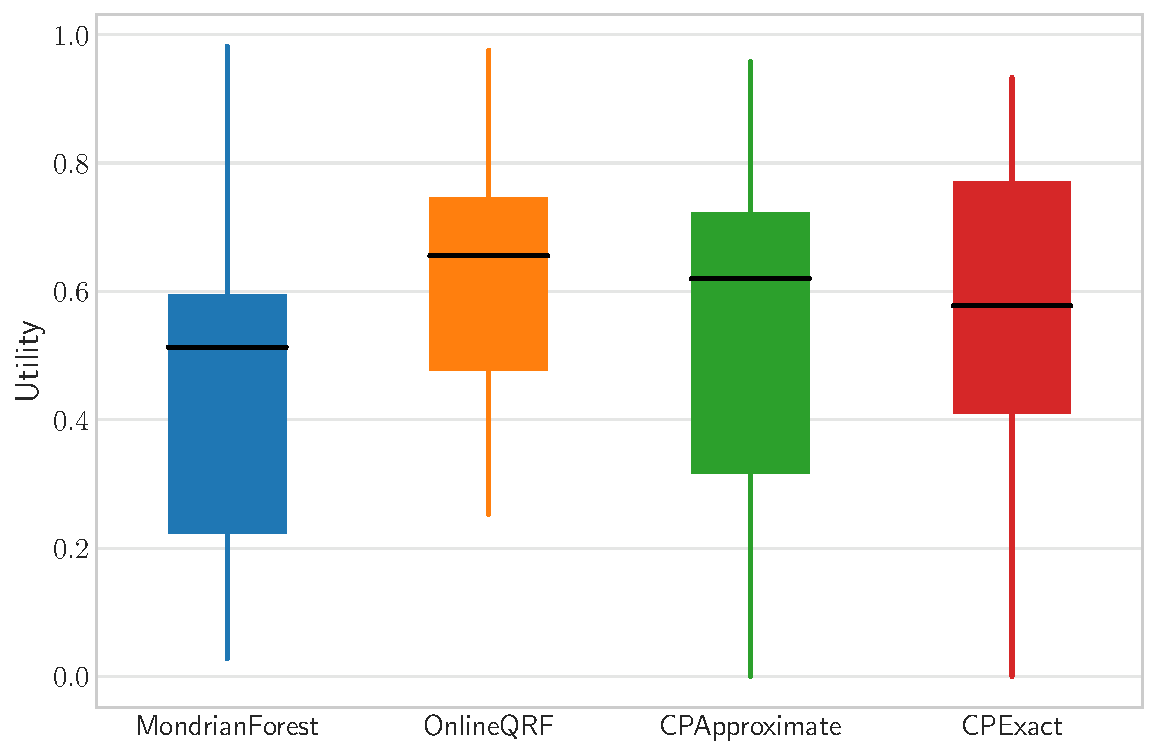
\includegraphics[width=0.8\columnwidth]{utility-small-mid}
	\caption{Utility for the small-scale data. Higher is better.}
	\label{fig:utility-small-mid}
\end{figure}

\begin{figure}
	\centering
	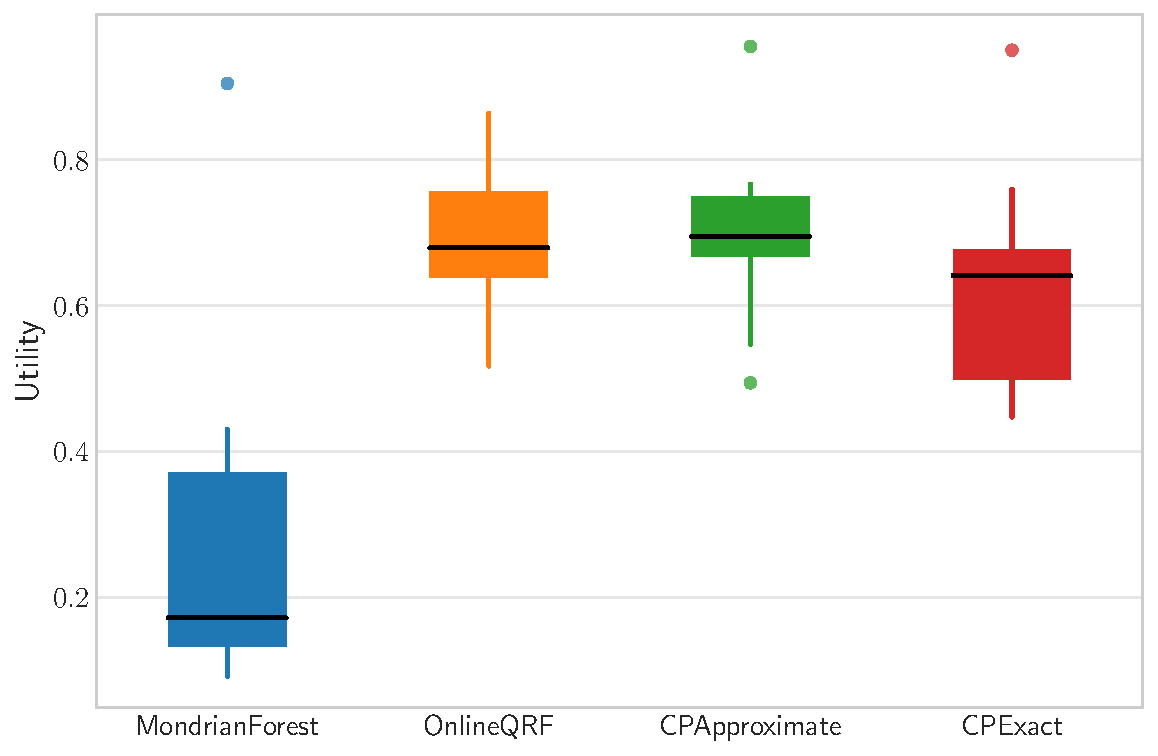
\includegraphics[width=0.8\columnwidth]{utility-concept_drift}
	\caption{Utility for the concept drift data. Higher is better.}
	\label{fig:utility-concept-drift}
\end{figure}

We also provide an evaluation for different significance levels.
Depending on the cost of making a mistake, we might require different levels of confidence
in our predictions. Thereby it's important to measure the performance of the
algorithms over a range of different significance levels. The results are listed
in Table \ref{tab:uncertain-significance} where we can see that Mondrian Forests cannot maintain the
error guarantees above 80\% confidence, and that OnlineQRF provides the best
compromise between maintaining the error rate below the requested level, while
keeping the produced intervals informative.

\begin{table}
	\centering
	\begin{tabular}{ll r r r r r}
		\toprule
		\multirow{2}{*}{Method} &  \multirow{2}{*}{Metric} &  \multicolumn{5}{c}{$\alpha$} \\
		\cmidrule(lr){3-7}
		& & 0.3 &   0.2 &   0.1 &   0.05 &   0.01 \\
		\midrule
		\multirow{2}{*}{MondrianForest}   & MER  & 0.28 & 0.20 & 0.13 &  0.094 &  0.062 \\
		& RIS  &  0.19 &  0.23 &  0.29 &   0.349 &   0.460 \\
		\midrule
		\multirow{2}{*}{OnlineQRF} & MER & 0.23 & 0.14 & 0.07 &  0.036 &  0.015 \\
		& RIS &  0.20 &  0.23 &  0.31 &   0.345 &   0.510 \\
		\midrule
		\multirow{2}{*}{CPApprox} & MER  & 0.22 & 0.13 & 0.06 &  0.032 &  0.006 \\
		& RIS &   0.21 &   0.31 &   0.48 &   0.785 &    1.130 \\
		\midrule
		\multirow{2}{*}{CPExact} & MER  & 0.25 & 0.16 & 0.08 &  0.039 &  0.009 \\
		& RIS &   0.28 &   0.37 &   0.57 &   0.622 &   0.944 \\
		\bottomrule
	\end{tabular}
	\caption{MER and RIS for different significance levels. The MER should be at most
		$\significance$ where $\significance$ the significance level.}
	\label{tab:uncertain-significance}
\end{table}

\section{Discussion}
\label{sec:uncertain-trees-discussion}

In this chapter we have presented our work on uncertainty estimation for
online decision trees. We developed two algorithms for this purpose,
and demonstrated their accuracy and efficiency compared to a state
of the art algorithm.

Connecting this work to our original goals in Section \ref{sec:intro-question-objectives},
we have dramatically reduced the computation necessary for online conformal
prediction by maintaining up-to-date online models. For both OnlineCP and
OnlineQRF we have bounded the memory use of the algorithms by using approximate
and bounded data structures, that are able to provide the estimates we need
at a fraction of the memory cost.
The approximations made however create a tradeoff,
as we can no longer guarantee the consistency and validity of the algorithms.
As the trees in a random forest are trained independently there is no
need to communicate model updates when running the algorithms in parallel.
However, for OnlineQRF in a distributed setting we would need to merge the histograms of each tree to provide
a quantile prediction. Through our use of the near-optimal KLL sketch we ensure
that the communication cost is minimal.
The optimizations listed cover two of the three objectives
listed in Section \ref{sec:intro-question-objectives} and this work investigates
an aspect of our research question in the context of uncertainty estimation.
\newpage
\chapter{Scalable Boosted Trees for High-dimensional Data}
\label{ch:boosted-trees}

In this chapter we provide an overview of our work on scaling boosted tree
learning. We tackle the problem in two different domains: online boosting
(\boostvht) and batch gradient boosting (\blockgbt). We develop algorithms
that are optimized for the distributed setting 

\section{Background}
\label{sec:scalable-boosted-background}

% Describe the problem
Boosting algorithms are some of the most successful and widely used algorithms
in machine learning, due to their simplicity and excellent accuracy. As a result,
a wide array of research has been proposed with the aim of improving the scalability
of boosting, either through parallelizing the base algorithm, or by developing
algorithms that can perform boosting online.

% Previous approaches and why they don't work
However, when it comes to high dimensional data current approaches fall short
in terms of scalability.
In the online domain, due to the sequential nature of online boosting algorithms,
current online methods do not make use of parallelism for training~\cite{online-gradient-boosting, Oza2001online, online-boosting-theoretical}.
On the other hand, existing methods for the batch
domain provide parallelism along only the data point dimension, limiting their
scale-out capabilities. As a result, for high-dimensional data with millions
of features, we are left with few choices: In the online domain there exist
no parallel algorithms, while in the batch domain the existing feature-parallel
algorithms make the assumption that the entire dataset can fit in the memory
of each worker, severely limiting the size of the problems we can tackle
\cite{lightgbm, xgboost}.

% Our method
In our work we tackle each domain separately:
In \boostvht, we enable parallelism in the online learning setting, while maintaining the guarantees of existing
online boosting algorithms. To achieve that, we use a sequential ensemble of model-parallel learners that train
on different parts of a single data point in a distributed environment.
In the batch domain we enable scalability across \emph{both} the data point and
feature dimensions by developing a block-distributed gradient boosted tree algorithm.
We provide algorithms that make block-distributed training feasible and communication-efficient.

\section{Online and Distributed Boosted Trees}
\label{sec:boostvht-method}

In \boostvht we make parallel online boosting possible, while maintaining the
correctness of the online boosting algorithms, by using feature-parallel. 
We make use of the Vertical Hoeffding Tree (VHT) algorithm \cite{kourtellis2016vht} which is a model-parallel
extension of the online Hoeffding tree algorithm \cite{vfdt}, often referred to as
Very Fast Decision Tree (VFDT)\todo{Make sure we have talked about the VFDT in the background}.
The VFDT algorithm will sort instances down the tree and update the statistics for the
leaf the instance ends up in. This separation of duties allows for the scalable design of
VHT: the algorithm uses two components, one called the \emph{model aggregator}
that is responsible for sorting instances to leafs and maintaining the model, and
one called the \emph{local statistics}, which are potentially many workers responsible
for maintain the statistics for the leaves of the tree.
The model aggregator is responsible for breaking up each instance into its constituent
features, and sending them, along with the label, to the local statistics workers.
The model aggregator will periodically query the local statistics to check if we have
collected enough information to split the leaf with high confidence, as done in the
original VFDT.

Our method makes use of the VHT,
and proposes optimizations that make the learning process efficient in a distributed
setting. We use a design that is similar to the original VHT in that we maintain
two main components, one model aggregator and local statistics. However, our model
aggregator hosts a sequential chain of VHT models, though which we pass each example.
This design allows us to maintain the sequential nature of the boosting algorithm,
and as a result the guarantees of any online boosting algorithm, while performing
the training in parallel and asynchronously in a set of local statistics workers.

We propose three optimizations over the original VHT algorithm to improve its
characteristics for distributed boosting. First, we design our local statistics
so that the same worker can host statistics from multiple member of the ensemble.
This enables to decouple the level of parallelism from the number of learners
in the ensemble, separating the algorithm's functional (speedup) and non-functional
(accuracy) constraints.
Second, this enables us to host the statistics for a range of features on the same
worker, across all the ensemble. This makes our communication pattern efficient:
We only need to send $p$  messages per instance, where $p$ is the chosen
parallelism level, compared to sending $m$ messages, where $m$ the
number of features. This will dramatically
reduce the number of messages sent, since we expect $m \gg p$. In addition, compared to existing
parallel boosting methods like AdaBoost.PL \cite{adaboost-pl} that need to communicate the complete
models between update, we only need to communicate the split decisions which are
much more compact.
Finally, our approach allows us to send each attribute slice only once to
each worker, as it suffices for each subsequent learner after the first
to only send their updated weight. This brings a communication reduction
of a factor $s$, where $s$ is the ensemble size, which can often be hundreds of
trees~\cite{hundreds-classifiers}.

\section{Block-distributed Gradient Boosted Trees}
\label{sec:block-gbt}

In \blockgbt we extend distributed gradient boosted trees, by parallelizing their
training across both the data point and feature dimensions, making use of block-distribution.
Here we provide a summary of each part of the training algorithm that we had to
adapt to the block-distributed setting.
The training process of GBTs can roughly be divided into three stages: First comes
the prediction part, in which we use the existing ensemble to make a prediction
for each point in the dataset. We use these predictions to get the gradient
value for each data point. Second comes the gradient histogram creation.
In this stage we use the computed gradients to create gradient histograms
for every feature, one for each leaf in the tree. A gradient histogram
for a feature contains in each bucket the sum of the gradients that corresponds to
that feature range. Finally, given the gradient histograms for each feature,
we have a final step of split selection, where we use these histograms to greedily
select the optimal split for each leaf.

\subsection{Block-distributed prediction}
\label{subsec:block-gbt-prediction}

In the row-distributed setting, each worker has access to all the features for the
horizontal slice of the data they are responsible for. This allows us them to determine
the exit node for each local data point without any communication.
That is not the case however
for block-distributed data where each worker only has access to parts of each data
point. In this case, when the model contains internal nodes that correspond to features
that are not present in one worker, they will need to communicate with the other
workers responsible for the same horizontal slice to determine the exit nodes.
What we want to avoid in this scenario is shuffling the data between workers,
as we could have millions of features leading to impractical communication
costs. In our approach we develop a novel use of the Quickscorer \cite{quickscorer} algorithm
that gives us provably correct and efficient block-distributed predictions.

Briefly, in Quickscorer the exit node can be determined by applying the bit-wise
\AND operation between specific bit-strings for every internal node.
These bit-strings are of length $|L|$, where $L$ the set of leaves, and
every zero indicates that a leaf node becomes impossible to reach if the node's
condition evaluates to false, and all other elements are one. When determining
the exit node for a particular example, we need to identify all the nodes in
the tree that evaluate to false for that example, and aggregate their bit-strings into one overall
bit-string \bitstring.
\citet{quickscorer}
prove that the left-most bit set to one in \bitstring will indicate the exit node for the example.

We adapt the above algorithm to work in the block-distributed setting. Each worker
now only has access to particular range of features for a subset of the data points.
So it an only evaluate the conditions of the tree that correspond to its slice
of the features. We create local bit-strings at each worker, one for each example.
These bit-strings have the same properties as in the original Quikscorer algorithm,
however can only eliminate leafs that are children of internal nodes that correspond
to the features available at that worker. To fully determine the output for each
data point, the workers that hold data for the same horizontal slice will need
to aggregate the bit strings for each data point. We do this by utilizing the
parameter server \cite{muPS} architecture\todo{Should have introduced the PS now, and
	esp. the server/worker concepts}: Each server is responsible for a
one horizontal slice of the data. The workers that hold the different parts of
a horizontal slice, all send their bit-strings to the same server.
The server then aggregates the partial bit-strings using a simple bit-wise \AND to determine the exit
node for each data point.

Because the \AND operator is both commutative and associative, the order in which
these aggregations happen does not affect the result, and the overall aggregation
will be equal to the aggregation of the partial aggregations. This ensures that
our predictions will be correct. By using this method we can determine the exit
nodes for each data point, and from that the corresponding gradients that we need
for the next step of histogram aggregation.

\subsection{Histogram Aggregation}
\label{subsec:block-gbt-histogram-aggregation}


With centralized data the histogram aggregation step requires no communication,
and can be performed by running a simple local aggregation.
For example, assume that for a specific leaf we have two data points, $\{x_1, x_2\}$,
and our dataset has two features $\{f_1, f_2\}$ each so that $x_1: \{0.1, 7\}$ and $x_2: \{1.5, 8\}$.
Say the gradient values of the data points are $\{x_1: 3.5, x_2: 0.5\}$.
The gradient histograms' buckets are determined by the empirical distribution of each
feature across the complete dataset. These are computed using a \emph{quantile sketch}
of the Cumulative Distribution Function for each feature. These are the same kind of sketches
as used in Chapter \ref{ch:uncertain-trees} for OnlineQRF. We choose a the number of split-points
$B$ we want to examine for each feature, and create equi-weight buckets for each feature
by iterating through the complet dataset. These calculated independently at each worker
and are then aggregated across the cluster to get the combined CDF for each feature.
In this example say we have two buckets:
$f_1: \{[0.0, 1.0), [1.0, 5.0)\}$ and $f_2:\{ [0.0, 5.0), [5.0, 10.0)\}$.
Then, for this leaf, the feature histogram for $f_1$ would be $\{3.5, 0.5\}$ and for $f_2$
it would be $\{0.0, 3.5 + 0.5\}$, since both data points have values for $f_2$ that fall
in the second bucket, $[5.0, 10.0)$, of the gradient histogram.

Now assume that we have a distributed dataset, and that $x_1$ resided on worker $w_1$ and $x_2$ resided on worker $w_2$. This is
an example of the row-distributed pattern that all current distributed algorithms assume.
In this case we need to create at each worker local histograms, which
in this case would be $f_1: \{3.5, 0.0\}$ and $f_2: \{0.0, 3.5\}$ for $w_1$, and $f_1: \{0.0, 0.5\}$ and $f_2: \{0.0, 0.5\}$ for $w_2$. To get a complete picture of the gradient histograms
we need to aggregate them between the workers, so the algorithm involves one communication
step. One drawback of all current row-distributed methods is that they use dense communication
for the aggregation we just described. For the example given above, dense communication
requires us to communicate $|F| \cdot B$ values for each worker, where $F$ the set of features,
and $B$ the number of histogram buckets. However,
many of the histogram values can be zero, as was the case for four out of the eight possible
values in the example. This problem is exacerbated when we are dealing with sparse
datasets with millions of features.

Block-distribution introduces another level of complexity into this operation, as
in that case, no worker has a complete view of any data point. Each worker gets one block,
that is, a horizontal \emph{and} vertical slice of the data. If we think of the complete
gradient histograms as a tensor of dimensions $|L| \times |F| \times B$, each worker is
will populate a part of this tensor, across the $L$ and $B$ dimensions, but limited to a specific
subset of $F$. In \blockgbt, we use a sparse representation of this tensor at each worker, which allows
us to eliminate the extraneous communication described above. Our experiments show
that for sparse datasets this brings down the communication cost by multiple orders
of magnitude.

Once each worker iterates
through their block of data, they send their partial tensor to one server. Each server
is now responsible for a range of features, so workers that belong to the same vertical
slice of data will send their tensors to the same server. Each server ends up having
a full view of the gradient histograms for a subset of features. The split finding step
can then be performed using an algorithm similar to the one proposed in \citet{dimboost}.

\section{Main Findings}

In this section we present the evaluation of the online distributed tree boosting
algorithm from \boostvht and the block-distributed GBT algorithm from \blockgbt.

\subsubsection*{Online and Distributed Boosted Trees}
\label{sec:boostvht-results}

For our online learning experiments we use 10 artificial and 4 real-world datasets. The artificial
datasets are generated with different numbers of attributes using one generator
from a tree-like structure, one that generates random tweet text for a sentiment
analysis task, and one rotating hyperplane. The baselines we test against are
a single-threaded online boosting algorithm from the MOA \cite{bifet2010moa}
library using the Hoeffding tree as a base learner, and the base VHT tree.
We measure the speedup over the single-threaded algorithm, and use the
robust Kappa\cite{bifet2015efficient} statistic to measure accuracy,
that considers the probability of agreement by chance in the evaluation.

We start by showing that the boosted version of the algorithm performs
better than the base VHT. Figure \ref{fig:boostvht-textgen-accuracy} shows an example experiment using different
levels of dimensionality for the text-generator data. We can see
that as we increase the number of features and make the problem more
difficult, the accuracy of the VHT algorithm deteriorates, while
BoostVHT is consistently accurate, and is practically equivalent to the single-threaded
boosting algorithm. At the same time the concurrent and parallel design of the algorithm
provides us with a speedup of \textbf{45$\times$} on average, compared to the single-threaded
implementation of MOA.

\begin{figure*}
	\centering
	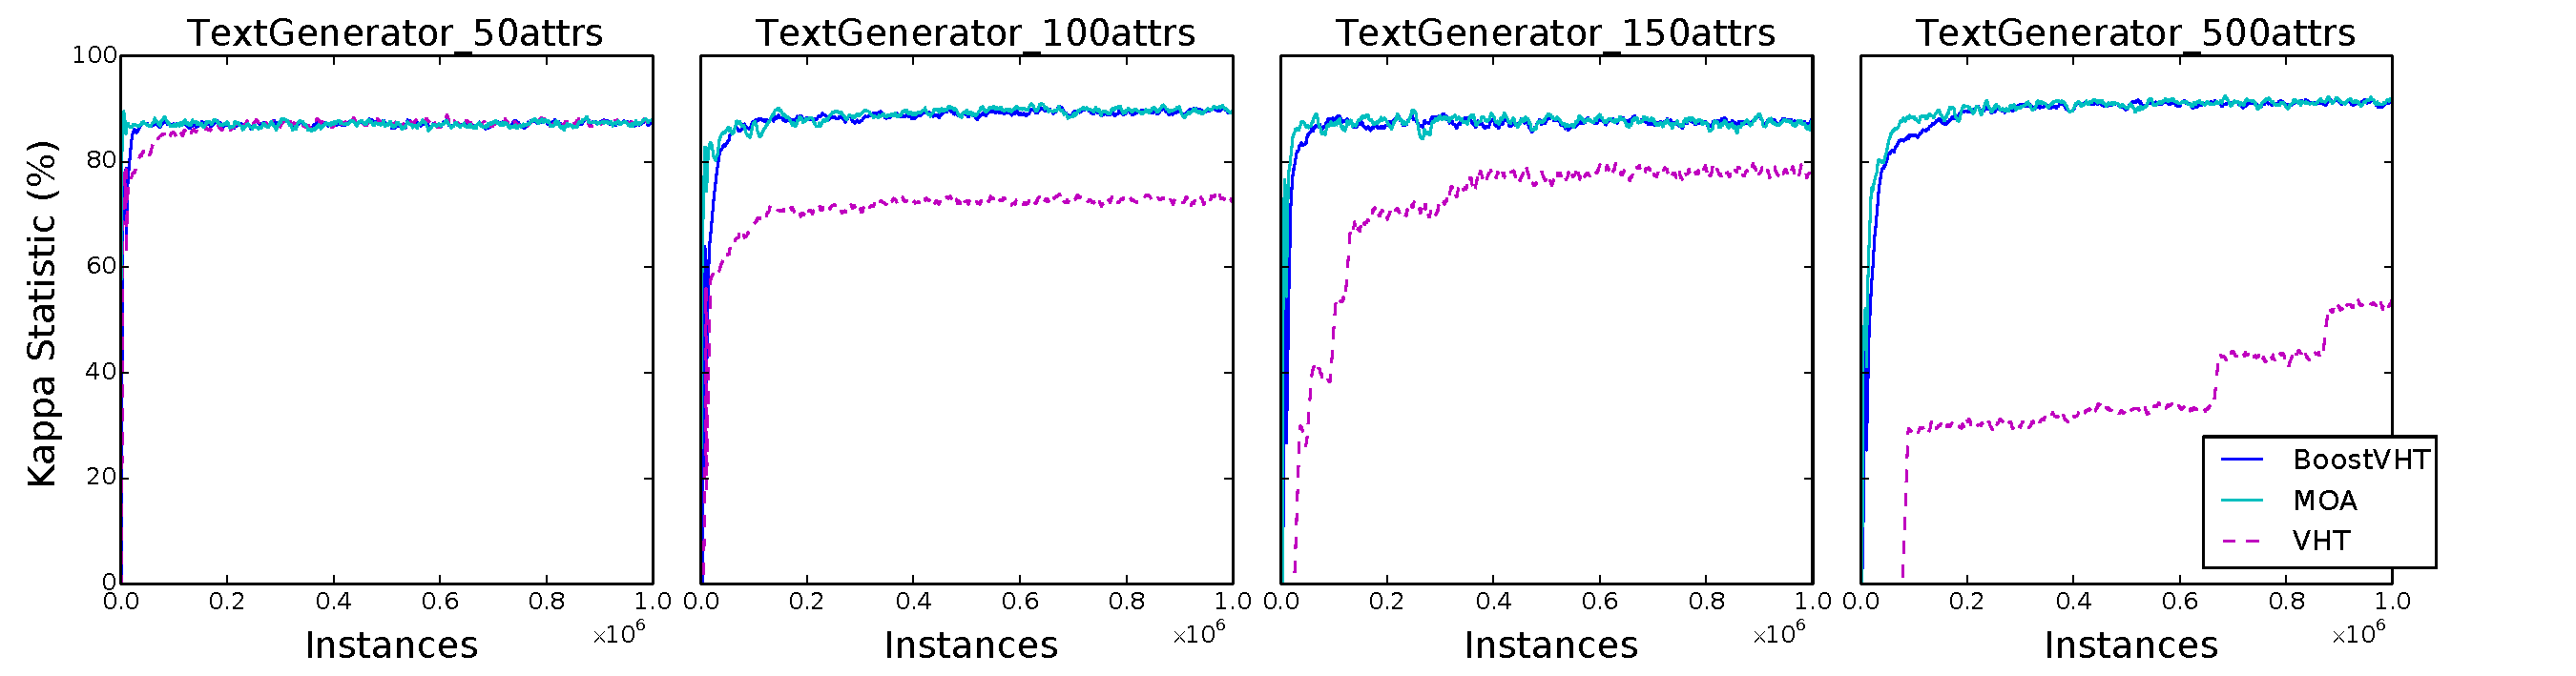
\includegraphics[width=\textwidth]{textGen_all_kappa_stat_storm.pdf}
	\caption{Kappa statistic (accuracy) as a function of arriving instances over time for text generator datasets with
		an increasing number of attributes.}
	\label{fig:boostvht-textgen-accuracy}
\end{figure*}

Finally we examine the scalability of the algorithm in terms of strong and weak scaling.
Ideal strong scaling provides \emph{linear speed-up}: Doubling the amount of resources
while keeping the problem size constant should halve the execution time.
Ideal weak scaling should have \emph{linear scale-out}: doubling both the problem size
and resources at the same time should affect the training time significantly.
We illustrate the scaling characteristics of the algorithm in Figures
\ref{fig:weak-scaling} and \ref{fig:strong-scaling} for weak and strong
scaling respectively. As we can see in the figures, the algorithm scales
almost ideally both in terms of weak scaling, keeping its training time
close to constant as we double resources and the problem size, and provides
near-linear speed-up for our strong scaling experiments.

\begin{figure}
	\centering
	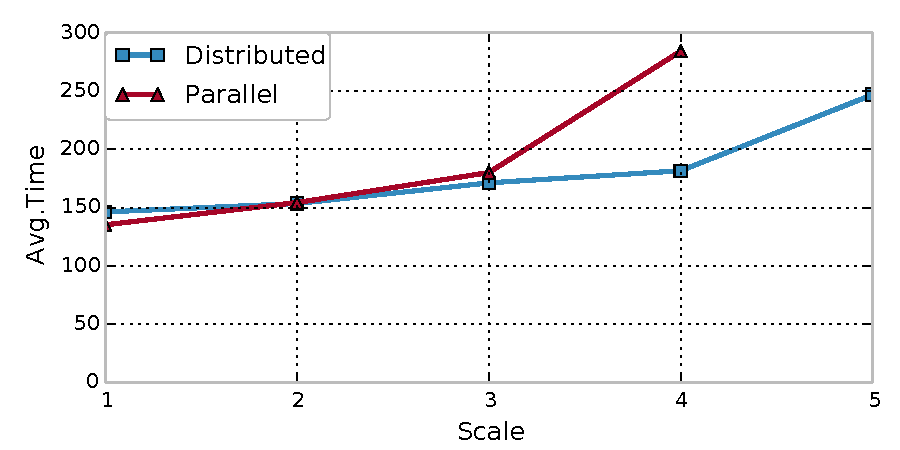
\includegraphics[width=0.8\textwidth]{weak-scaling.pdf}
	\caption{Weak scaling experiments, time in milliseconds. Scale 1x on the x-axis refers to 500 attributes with 2 Processors, and we double both Processors and attributes for each scale increment (up to 8,000 attributes with 32 Processors).}
	\label{fig:weak-scaling}
\end{figure}

\begin{figure}
	\centering
	\begin{subfigure}[t]{0.5\textwidth}
		\centering
		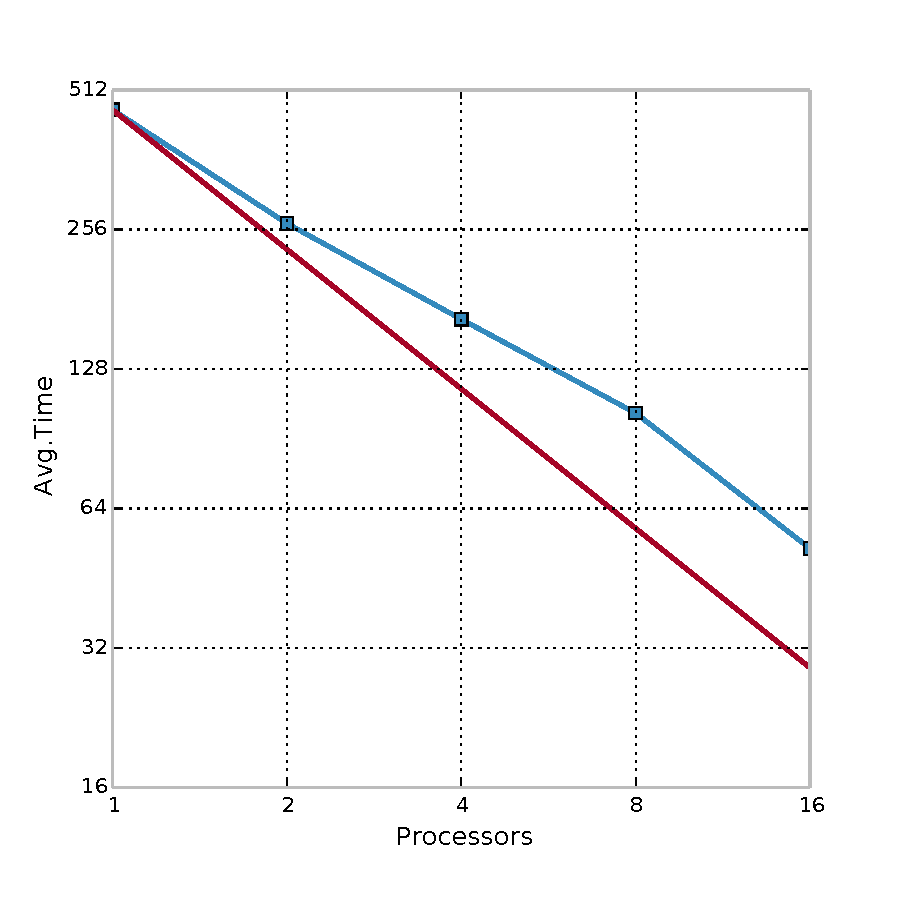
\includegraphics[width=\linewidth]{ice-strong-scaling.pdf}
		\caption{Parallel experiments.}
		\label{fig:strong-parallel}
	\end{subfigure}%
	\begin{subfigure}[t]{0.5\textwidth}
		\centering
		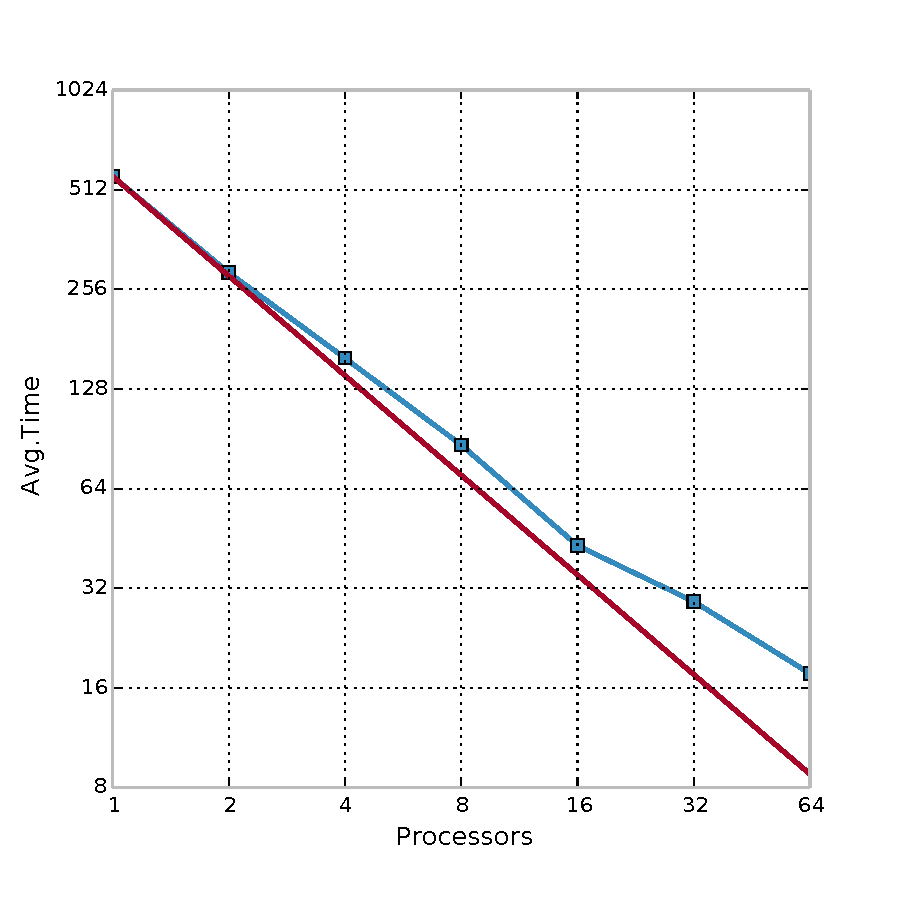
\includegraphics[width=\linewidth]{ec2-strong-scaling.pdf}
		\caption{Distributed experiments}
		\label{fig:strong-distributed}
	\end{subfigure}
	\caption{Strong scaling in the parallel (left) and distributed (right) setting. The
		time reported is the average time to train 1,000 instances, each with 1,000 attributes, in milliseconds. The red straight line indicates ideal linear scaling.}
	\label{fig:strong-scaling}
\end{figure}

\subsubsection*{Block-distributed Gradient Boosted Trees}
\label{sec:block-gbt-results}

To determine the performance gains and limitations of block-distributed approach and
the sparse communication we use 4 datasets with different sparsity levels. First
we have two highly sparse datasets, URL and avazu with roughly 3,2 million and
1 million features respectively. Second we use the RCV1 dataset with approximately
47 thousand features and the dense Bosch dataset with 968 features. 

We measure the
communication cost in MiB for the dense histograms of the row-distributed approach
and our sparse block-distributed histograms. We also evaluate the end-to-end runtime
of the histogram aggregation step, divided into communication and computation stages,
to measure the real-world runtime. This step is the most computationally intensive
part of GBT learning \cite{comm-efficient-gbt} and in our experiments constitutes
at least 90\% of the total runtime.

In Figure \ref{fig:block-gbt-hist-size} we can see the benefits of sparse communication:
For the highly sparse URL and avazu datasets the reduction in communication is five and three orders of magnitude respectively. The sparse histograms however introduce additional computational
cost: unlike dense data structures that are contiguous in memory, sparse structures use
indirect addressing which makes building and accessing these histograms cache-unfriendly.
This, in combination with the overhead introduced by the use of the parameter server
leads to increased computation time.
While in sparse datasets the significant gains made by minimizing the communication time
allows us to compensate for the increased computation, that is not the case for
the dense data, where computation time dominates, as shown in Figure \ref{fig:block-gbt-time}.


\begin{figure}
	\centering
	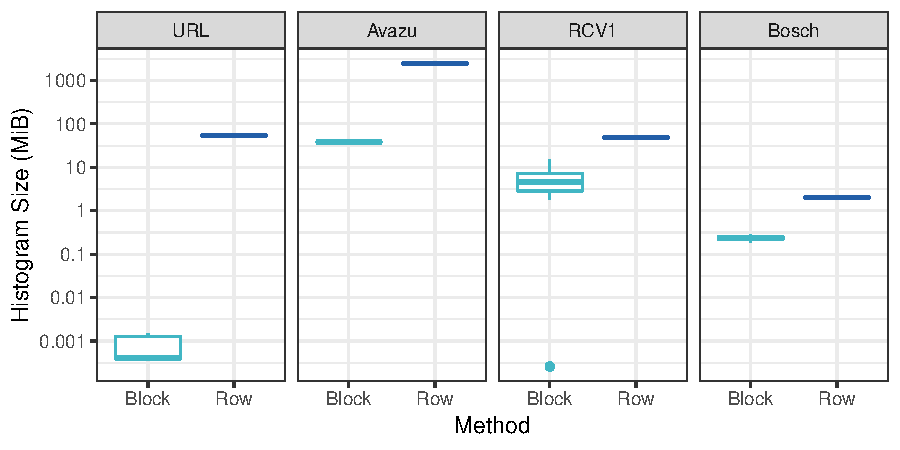
\includegraphics[width=0.8\textwidth]{block-gbt-hist-box.pdf}
	\vspace{-10pt}
	\caption{The byte size of the gradient histograms being communicated for the various datasets.}
	\label{fig:block-gbt-hist-size}
\end{figure}

\begin{figure}
	\centering
	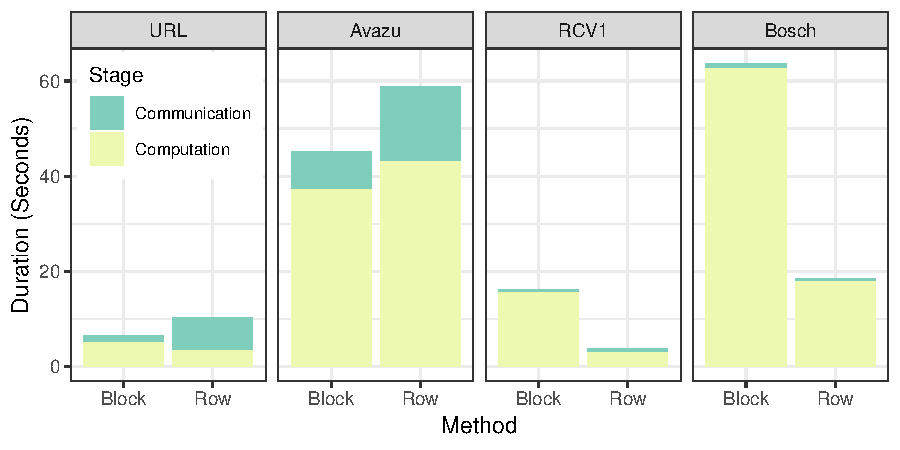
\includegraphics[width=0.8\textwidth]{block-gbt-time.pdf}
	\vspace{-10pt}
	\caption{The communication and computation times for the various datasets, in seconds.}
	\label{fig:block-gbt-time}
\end{figure}


Finally we demonstrate the communication savings possible in terms of the feature sketches. As we mentioned in Section \ref{sec:uncertain-trees-background}, in order to determine the possible
split points for each feature, we need to have an estimate of the CDF for each feature. These
can be calculated once at the beginning of learning, or once per leaf, to get a more accurate representation
of the CDF in every leaf. \citet{xgboost} show that generating per-leaf (local) split points leads to the same overall
accuracy as using the overall sketches (global) while using much less accurate sketches, thereby creating potential communication savings:
A quantile sketch's size is determined by the level of error in the approximation we can
accept \cite{karnin2016kll}.

However, when using dense communication we need to know the size
of the sketch being communicated in advance. In a probabilistic sketch, this is only possible
if we use the maximum theoretical size of a sketch, to ensure the sketches do not overlap in memory.
This of course is a major source of inefficiency, as the actual size of the sketches can be orders
of magnitude smaller. For this reason
current distributed approaches all use the global sketch approach, in order to only communicate
the sketches once at the beginning of learning instead of having to communicate once for every
leaf.

Using our sparse approach however, allows us to only communicate the true size of the sketches,
thereby providing massive savings in communication, as shown in Figure \ref{fig:block-gbt-sketch-size}. This would allow the sketches to be communicated for every
leaf, leading to even further savings by using lower accuracy sketches or increased accuracy
in the CDF representation.

\begin{figure}
	\centering
	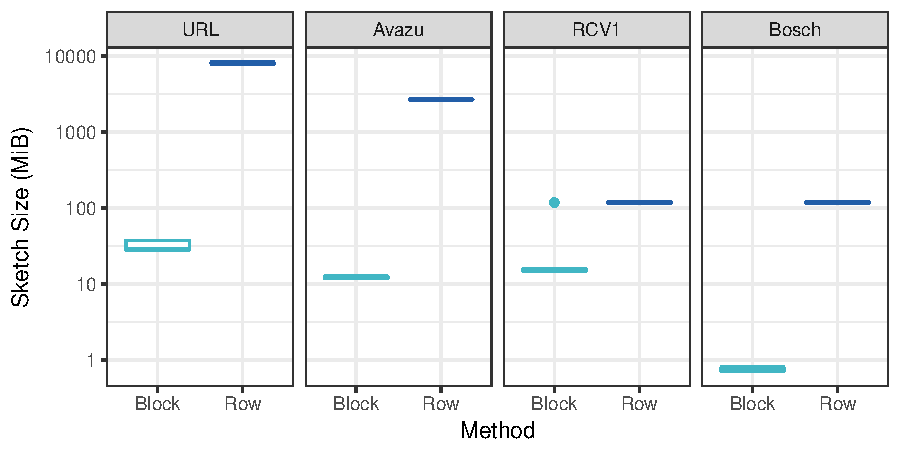
\includegraphics[width=0.8\textwidth]{block-gbt-sketch-box.pdf}
	\vspace{-10pt}
	\caption{The byte size of the feature sketches being communicated for the various datasets.}
	\label{fig:block-gbt-sketch-size}
\end{figure}
\newpage
\part{Concluding Remarks}
\label{part:conclusion}
\chapter{Conclusion}

\section{Summary of Results}

\section{Future Directions}
\newpage

\backmatter
\printindex
%\printreferences

\bibliographystyle{kthnat} % this is just an example, other styles can be used as well
\bibliography{main} % calls the separate document named Doc.bbl

\end{document}
